%You can leave alone everything before Line 79.
\documentclass{article}
\usepackage{url,amsfonts, amsmath, amssymb, amsthm,color, enumerate, verbatim}
% Page layout
\setlength{\textheight}{8.75in}
\setlength{\columnsep}{2.0pc}
\setlength{\textwidth}{6.5in}
\setlength{\topmargin}{0in}
\setlength{\headheight}{0.0in}
\setlength{\headsep}{0.0in}
\setlength{\oddsidemargin}{0in}
\setlength{\evensidemargin}{0in}
\setlength{\parindent}{1pc}
\newcommand{\shortbar}{\begin{center}\rule{5ex}{0.1pt}\end{center}}
%\renewcommand{\baselinestretch}{1.1}
% Macros for course info
\newcommand{\courseNumber}{ME 552}
\newcommand{\courseTitle}{Mechatronics}
\newcommand{\semester}{Fall 2012}
\newcommand{\xxx}[1]{\textcolor{red}{#1}}
% Theorem-like structures are numbered within SECTION units
\theoremstyle{plain}
\newtheorem{theorem}{Theorem}[section]
\newtheorem{lemma}[theorem]{Lemma}
\newtheorem{corollary}[theorem]{Corollary}
\newtheorem{proposition}[theorem]{Proposition}
\newtheorem{statement}[theorem]{Statement}
\newtheorem{conjecture}[theorem]{Conjecture}
\newtheorem{fact}{Fact}
%definition style
\theoremstyle{definition}
\newtheorem{definition}[theorem]{Definition}
\newtheorem{example}{Example}
\newtheorem{problem}[theorem]{Problem}
\newtheorem{exercise}{Exercise}
\newtheorem{algorithm}{Algorithm}
%remark style
\theoremstyle{remark}
\newtheorem{remark}[theorem]{Remark}
\newtheorem{reduction}[theorem]{Reduction}
%\newtheorem{question}[theorem]{Question}
\newtheorem{question}{Question}
%\newtheorem{claim}[theorem]{Claim}
%
% Proof-making commands and environments
\newcommand{\beginproof}{\medskip\noindent{\bf Proof.~}}
\newcommand{\beginproofof}[1]{\medskip\noindent{\bf Proof of #1.~}}
\newcommand{\finishproof}{\hspace{0.2ex}\rule{1ex}{1ex}}
\def\therefore{\boldsymbol{\text{ }
\leavevmode
\lower0.4ex\hbox{$\cdot$}
\kern-.5em\raise0.7ex\hbox{$\cdot$}
\kern-0.55em\lower0.4ex\hbox{$\cdot$}
\thinspace\text{ }}}

\newenvironment{solution}[1]{\medskip\noindent{\bf Problem #1.~}}{\shortbar}

%====header======
\newcommand{\solutions}[4]{
%\renewcommand{\thetheorem}{{#2}.\arabic{theorem}}
\vspace{-2ex}
\begin{center}
{\small  \courseNumber, \courseTitle
\hfill {\Large \bf {#1} }\\
\semester, University of Michigan, Ann Arbor \hfill
{\em Date: #3}}\\
\vspace{-1ex}
\hrulefill\\
\vspace{4ex}
{\LARGE Lab Assignment #2}\\
\vspace{2ex}
\end{center}
\begin{trivlist}
\item \textsc{Team members:\\} {#4}
\end{trivlist}
\noindent
\shortbar
\vspace{3ex}
}
% math macros
\newcommand{\defeq}{\stackrel{\textrm{def}}{=}}
\newcommand{\Prob}{\textrm{Prob}}
\newcommand{\Lagr}{\mathcal{L}}
\newcommand{\Sens}{\mathcal{S}}
%==
\usepackage{graphicx}
\usepackage{xfrac}
\usepackage{amsmath}
\providecommand{\e}[1]{\ensuremath{\times 10^{#1}}}
\begin{document}
%%%%%%%%%%%%%%%%%%%%%%%%%%%%%%%%%%%%%%%%%%%%%%%%%
%\solutions{Your name}{Problem Set Number}{Date of preparation}{Collaborators}{Prover}{Verifiers}
\solutions{}{6: Inertial Sensors}{\today}{Shiva Ghose, @gshiva\\ John Peterson, @jrpeters\\ Peter Turpel, @pturpel\\ Chan-Rong Lin, @pmelin}
%%%%%%%%%%%%%%%%%%%%%%%%%%%%%%%%%%%%%%%%%%%%%%%%%
%\renewcommand{\theproblem}{\arabic{problem}} 
%%%%%%%%%%%%%%%%%%%%%%%%%%%%%%%%%%%%%%%%%%%%%%%%%
%
% Begin the solution for each problem by
% \begin{solution}{Problem Number} and ends it with \end{solution}
%
% the solution for Problem 
\section*{Teamwork Participation Pledge :: Team 1}

I attest that I have made a fair and equitable contribution to this lab and submitted 
assignment. \\

My signature also indicates that I have followed the University of Michigan Honor Code, 
while working on this lab and assignment.\\

I accept my responsibility to look after all of the equipment assigned to me and my team, 
and that I have read and understood the X50 Lab Rules.\\

\begin{table}[h]
\begin{center}
    \begin{tabular}{|c|c|c|}
        \hline
        \textbf{Name} & \textbf{Email}     & \textbf{ \ \ \ \ \  \ \  \ \ \ \ \  \ \ Signature  \ \ \ \ \  \ \ \ \ \ \ \  \ \ } \\ \hline
        	~& ~& ~\\
	~& ~& ~\\
	Shiva Ghose   & gshiva@umich.edu   & ~                  \\
	~& ~& ~\\
	~& ~& ~\\ \hline 
	~& ~& ~\\
	~& ~& ~\\
        John Peterson & jrpeters@umich.edu & ~                  \\ 
	~& ~& ~\\
	~& ~& ~\\ \hline 
	~& ~& ~\\
	~& ~& ~\\
        Peter Turpel   & pturpel@umich.edu & ~                  \\
	~& ~& ~\\
	~& ~& ~\\ \hline 
	~& ~& ~\\
	~& ~& ~\\
        Chan-Rong Lin   & pmelin@umich.edu & ~                  \\
	~& ~& ~\\
	~& ~& ~\\ \hline 
        \hline
    \end{tabular}
\end{center}
\end{table}

\newpage

\section{Accelerometer Wiring \& Configuration} 

\subsection{Configuration}

Figure \ref{wiring} shows the wiring diagram of the inertial sensor system. The accelerometer is mounted to a breadboard fixed to the the shaft clamp on the encoder such that the plane of the sensor PCB is perpendicular to the plane of axis of rotation of the encoder, shown later in figure \ref{sensorMount}.  This is necessary because of the limited number of axes available on the rate gyro.  For this assignment we will be making use of the Y and Z axes of the accelerometer and the X axis of the rate gyro (standard and X4.5). We also connected the auto-zero and temperature sensor pins. We are not using the X axis of the accelerometer, the Y axis of the rate gyro (standard and Y4.5), the self-test, or the VRef pins. We used an Arduino Uno as a voltage regulator to provide the encoder with 5V and the IMU with 3.3V.m the Arduino itself was powered from a wall outlet via an AC-to-DC converter.   \\

\begin{figure}[hbt]
\begin{center}
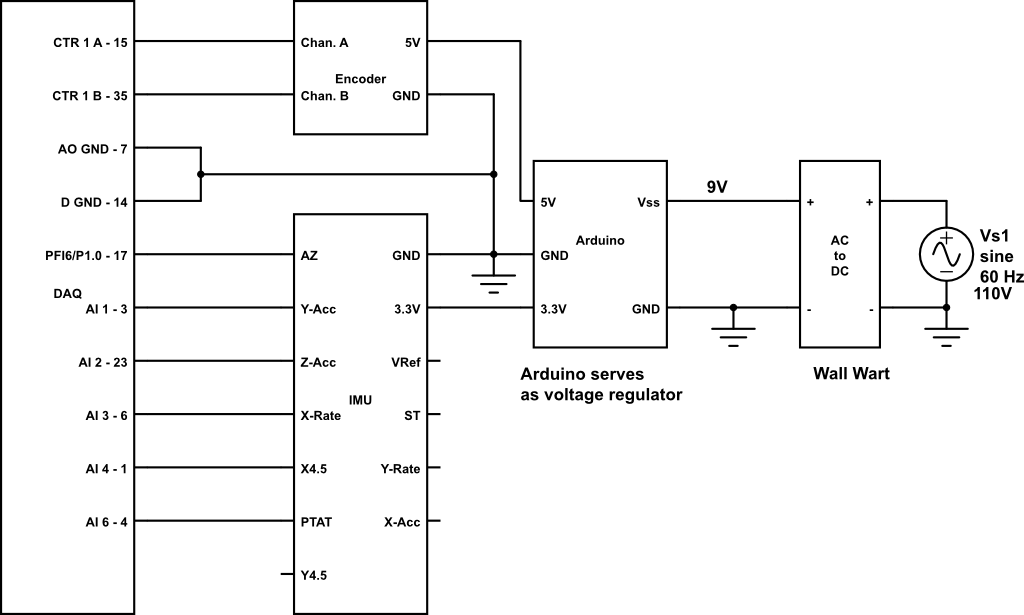
\includegraphics[width = 16cm]{WiringDiagram.png}
\caption{Wiring Connections of Inertial Sensor System.}
\label{wiring}
\end{center}
\end{figure}

\clearpage

\subsection{Pin Functionality}

\subsubsection{Accelerometer}
Figures \ref{accelPins} and \ref{accelFunc} show the arrangement of the pins on the accelerometer and its functional block diagram, respectively. \\

\begin{figure}[hbt]
\begin{center}
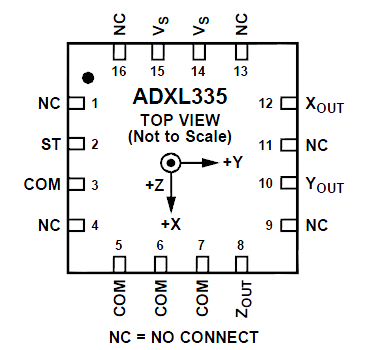
\includegraphics[width = 7cm]{ADXL335Pins.png}
\caption{Pin Configuration of the ADXL335 3-Axis Accelerometer.}
\label{accelPins}
\end{center}
\end{figure}

\begin{figure}[hbt]
\begin{center}
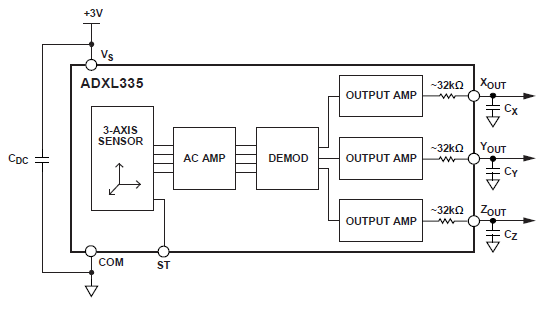
\includegraphics[width = 11cm]{ADXL335Functional.png}
\caption{Functional Diagram of the ADXL335 3-Axis Accelerometer.}
\label{accelFunc}
\end{center}
\end{figure}

\textbf{Pins 1, 4, 9, 11, 13, and 16 - NC}\\
These pins are not connected to the accelerometer's internal circuitry. They are not functional, but they can be connected to ground (the COM pins).\\

\textbf{ Pin 2 - ST}\\
This pin is for the self-test feature of the accelerometer. When the pin is set high by applying the supply voltage, an electrostatic force is applied to the accelerometer axes. This results in a known change in the voltage output from each axis. If the change is not seen in the output, this is an indication that there is a problem with the accelerometer. The pin can be connected to ground or left unconnected when not needed. The sparkfun PCB provides a connection for this pin, which we did not use.\\

\textbf{Pins 3, 5, 6, and 7 - COM}\\
These pins connect various elements of the accelerometer chip to ground. The PCB provides a connection for ground from the power supply and internally connects this to all of the COM pins. We connected this to the ground terminal of the Arduino.\\

\textbf{Pins 8, 10, and 12 - Z$_{out}$, Y$_{out}$, and X$_{out}$ (respectively)}\\ 
Analog voltage output of the 3 axes of the accelerometer. Each axis outputs voltage proportional to acceleration in that direction with a range of $\pm$ 3g according to equation \ref{Accel_EQ}.  According to the data-sheet, the Z axis accelerometer has greater noise density and lower bandwidth compared to the X and Y axes, which function identically. These parameters are noted in table \ref{ParamID_AccelT}.  The PCB provides connections for these pins. We connected pins 8 and 10 to the NI breakout board to read with LabView.  Pin 12 was left unconnected because the X-axis of the accelerometer is parallel to the axis of rotation of the encoder making it useless for reading angles.\\

\begin{equation}
V_{out} = V_{bias} + \Sens \ddot{u} \quad V_{bias} \approx \frac{V_{supply}}{2}
\label{Accel_EQ}
\end{equation}


\textbf{Pins 14 and 15 - V$_s$}\\
Supply voltage for the accelerometer. The accelerometer has a functional supply range of 1.8 V to 3.6 V, with a maximum range of -0.3 V to 3.6 V (based on operation reasonably safe from damage, not functional operation). The accelerometer is ratiometric with typical performance values given based on a V$_s$ of 3 V. Because the output is ratiometric, it is important to use a regulated power supply providing constant voltage. The PCB provides a connection for these pins, which we connected to the 3.3 V terminal of an Arduino Uno.\\ 

\subsubsection{Rate Gyro}
Figures \ref{gyroPins} and \ref{gyroFunc} show the arrangement of the pins on the rate gyro and its functional block diagram, respectively. \\

\begin{figure}[hbt]
\begin{center}
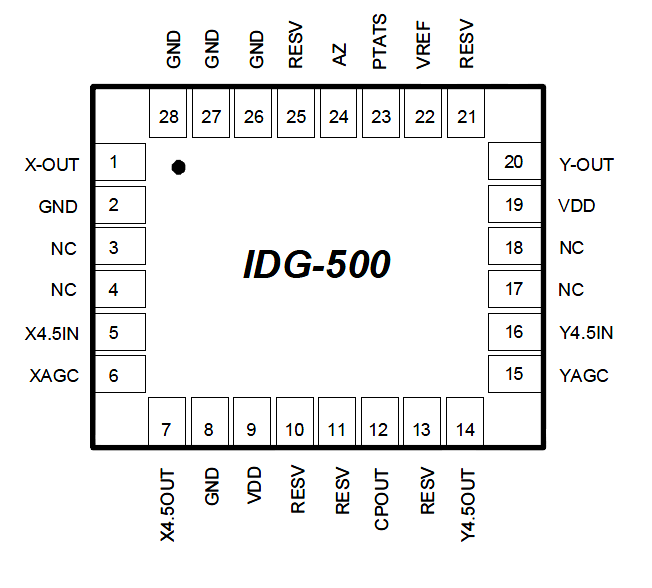
\includegraphics[width = 8cm]{IDG500Pins.png}
\caption{Pin Configuration of the IDG500 Dual-Axis Gyro.}
\label{gyroPins}
\end{center}
\end{figure}

\begin{figure}[hbt]
\begin{center}
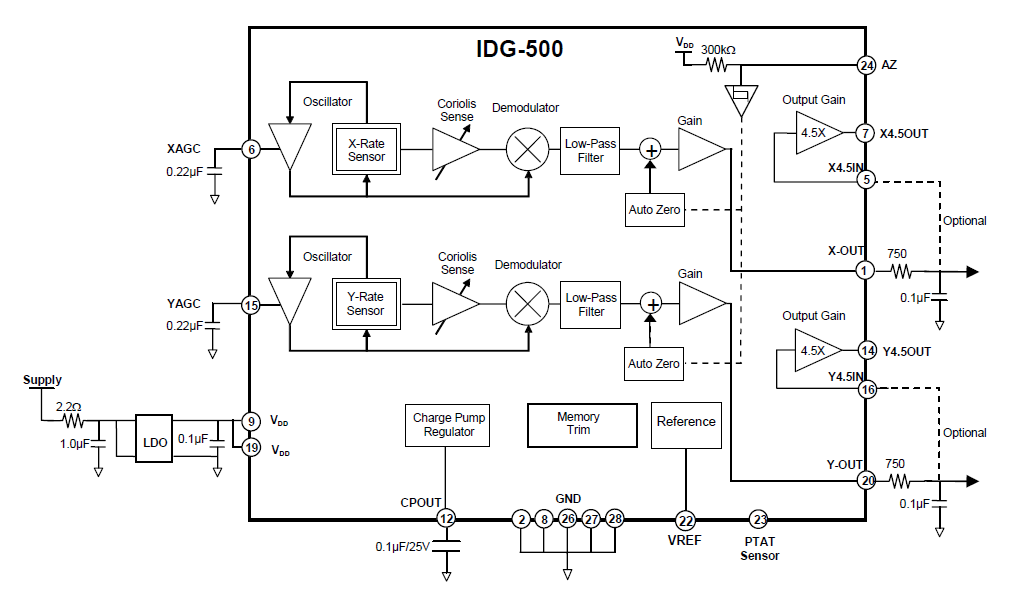
\includegraphics[width = 16cm]{IDG500Functional.png}
\caption{Functional Diagram of the IDG500 Dual-Axis Gyro.}
\label{gyroFunc}
\end{center}
\end{figure}

\textbf{Pins 1 and 20 - X-OUT and Y-OUT (respectively)}\\
Analog output voltage of the X and Y axes of the gyro. The gyro outputs voltage proportional to the angular rate about the X and Y axes according to equation \ref{RateGyro_EQ}. The outputs are not ratiometric and have a nominal full scale range of $\pm$500$^{\circ}$ and sensitivity of 2 $\frac{mV}{^{\circ}/s}$.  A low-pass filter is provided internally.  Additional parameters are described in table \ref{ParamID_DatasheetGyro}.  The PCB provides connections to these pins. We connected X-OUT to the NI breakout board to read with LabView, but did not connect Y-OUT because our setup did not rotate about that axis.\\

\begin{equation}
V_{out} = ZeroRate + \Sens_{Gyro} \dot{\theta} 
\label{RateGyro_EQ}
\end{equation}


\textbf{Pins 2, 8, 26, 27, and 28 - GND}\\
These pins connect various elements of the gyro chip to ground. The PCB provides a connection for ground from the power supply and internally connects this to all of the GND pins. We connected this to the ground terminal of the Arduino.\\

\textbf{Pins 3, 4, 17, and 18 - NC}\\
These pins are not connected to the gyro's internal circuitry. The data sheet notes that they can be used for PCB trace routing.\\

\textbf{Pins 5 and 16 - X4.5IN and Y4.5IN (respectively)}\\
These pins are inputs to amplifiers which can be connected to X-OUT and Y-OUT to provide higher sensitivity outputs. The connections are optional but are provided internally by the PCB.\\

\textbf{Pins 6 and 15 - XAGC and YAGC (respectively)}\\
These pins provide connections for amplitude control capacitors. 0.22 $\mu$F capacitors are internally used to connect these pins to ground. The capacitors are part of a control loop which controls the amplitude of the internal gains to ensure the sensitivity does not vary with temperature.\\

\textbf{Pins 7 and 14 - X4.5OUT and Y4.5OUT (respectively)}\\
Analog output voltage of the X and Y axes of the gyro. These pins increase the output of X-OUT and Y-OUT by a gain of 4.5 - effectively increasing the sensitivity at the expense of range. The output has a nominal full scale range of $\pm$110$^{\circ}$ and sensitivity of 9.1 $\frac{mV}{^{\circ}/s}$. The PCB provides connections to these pins. We connected X4.5OUT to the NI breakout board to read with LabView, but did not connect Y4.5OUT because our setup did not rotate about that axis.\\

\textbf{Pins 9 and 19 - VDD}\\
Supply voltage for the gyro. The gyro has a functional supply range of 2.7 V to 3.3 V, with a maximum range of -0.3 V to 6.0 V (based on operation reasonably safe from damage, not functional operation). The gyro is not ratiometric and all performance values are based on a VDD of 3 V. The PCB provides a connection for these pins, which we connected to the 3.3 V terminal of an Arduino Uno. A voltage regulator (likely a MIC5205) is included on the PCB betweent the VDD pins and the 3.3 V input connection to ensure the gyro receives 3.0 V. \\ 

\textbf{Pins 10, 11, 13, 21, and 25 - RESV}\\
These pins are reserved and are not connected.\\

\textbf{Pin 12 - CPOUT}\\
Provides an internal connection from ground to a charge pump regulator via a 0.1 $\mu$F capacitor. A charge pump is used for DC/DC regulation and can boost voltages without needing an inductor. \xxx{Might need more explanation here}\\

\textbf{Pin 22 - VREF}\\
A precision reference output which is nominally 1.35 V. Ideally VREF will be a constant 1.35 V and is used with the auto-zero function to reset the zero-rate output to its nominal value of 1.35 V in the event of steady-state drift. The PCB provides a connection to this pin which we did not use.\\

\textbf{Pin23 - PTATS}\\
Provides an output voltage from a temperature sensor within the gyro chip. Output is proportional to temperature with a nominal bias voltage of 1.25 V and a sensitivity of 4 mV/$^{\circ}$C. The PCB provides a connection to this pin which we connected to the NI breakout board and read in LabView (though we did not end up using the data).\\

\textbf{Pin 24 - AZ}\\
This pin is an input to an auto-zero funciton for the X and Y axis gyros. When activated, the auto-zero resets the zero-rate output to be equal to VREF. The auto-zero is typically used when the gyro is not moving to prevent steady-state drift and is supposed to increase the usable range of the high sensitivity outputs (X4.5OUT and Y4.5OUT). The auto-zero is intiated by setting the pin high with a pulse between 2 and 1500 $\mu$s. The PCB provides a connection to this pin with we connected to a digital output of the NI breakout board. In our LabView VI we connected a boolean momentary switch to this output so the user could activate the auto-zero, but this was rarely used.\\ 

\section{Modeling Assumptions}
% there is probably more stuff
While working with the system we made the following assumptions:
\begin{itemize}
\item{Assume that outputs of each axis of the accelerometer and the gyro are independent of one another}
\item{Assume zero bias of each accelerometer axis is stationary} % we may eliminate this assumption if we do online calibration
\item{$g = 9.81 \, \left( \sfrac{m^2}{s}\right) $}
\item The noise in the system is independent and identically distributed.
\item At start up the pendulum arm was facing down and an initial sensor calibration was performed each time.
\end{itemize}

\section{Parameter Identification}

\subsection*{Accelerometers}
The basic behavior of an accelerometer, sensitive in the $\hat{u}$ direction is given by equation \ref{ParamID_EQ1} for quasi-static accelerations.  Where $V_{out}$ is the output voltage of the sensor, $V_{bias}$ is the output of the sensor under no acceleration, $V_{supply}$ is the supply voltage to the sensor, and $\Sens$ is a linear approximation of sensor behavior.

\begin{equation}
V_{out} = V_{bias} + \Sens \ddot{u} \quad V_{bias} \approx \frac{V_{supply}}{2}
\label{ParamID_EQ1}
\end{equation}

This response to acceleration can be also be used to measure the acceleration due to gravity along the sensitive axis of an accelerometer allowing the angle between the accelerometer and vertical to be determined.  Let $\theta$ be the measured angle from vertical to the $\hat{y}$ direction of our system.  We can consider two situations, when the sensitive axis is aligned with $\hat{y}$ axis and when it is perpendicular to it.  Let $Y$ and $Z$ denote these situations respectively which correspond to the $\hat{y}$ and $\hat{z}$ axes of our accelerometer.  Then the output voltage of each axis is given as follows:

\begin{equation}
V_{Y} = V_{Ybias} + \Sens_{Y} g \cos(\theta) \quad V_{Z} = V_{Zbias} + \Sens_{Z} g \sin(\theta)
\label{ParamID_EQ2}
\end{equation}

\begin{figure}
\begin{center}
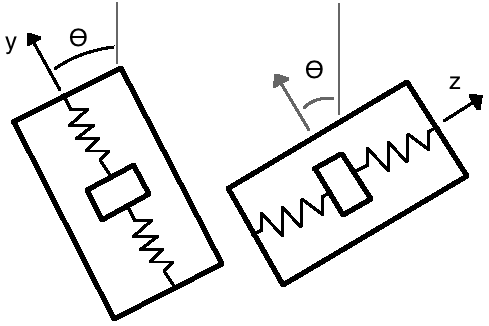
\includegraphics[width = 11cm]{Accelerometer_Cartoon.png}
\caption{Y and Z axis accelerometer}
\label{Accel_cartoon}
\end{center}
\end{figure}

We measured the bias voltage of each axis by fixing the accelerometer such that the axis was perpendicular to the force of gravity and recording the voltage output.  We obtained the bias voltage by averaging these voltages, and we also obtained a measure of noise along each axis by computing the variance of the obtained voltages.  We then conducted a simple experiment where the accelerometer was rotated at slow speeds throughout a complete circle while both axis voltage outputs and encoder angle measurements were recorded.  The equations in \ref{ParamID_EQ2} are linear in the sensitivity values, so we obtained each value through simple least squares regression.  These results are shown in table \ref{ParamID_T}. \\

The expected variance in voltage was computed using the bandwidth and noise density values given by the data-sheet for each axis according to the following equation.


$$\sigma = rms \, Noise = Noise \, Density \sqrt{BW * 1.6} $$

\begin{table}
\begin{center}
	\begin{tabular}{|c|c|}
		\hline
		Bandwidth $(Hz)$ & 50 \\ 
		Noise Density $Y_{out} \, \sfrac{\mu g}{\sqrt{Hz}} \, rms$ & 150 \\ 
		Noise Density $Z_{out} \, \left(\sfrac{\mu g}{\sqrt{Hz}} \, rms\right)$ & 300 \\ 
		Sensitivity $\left( \sfrac{mV}{g} \right)$ & 300 \\  
		$\sigma^2 \,Y_{out} \, (V^2)$ & $1.62 \e{-7}$ \\ 
		$\sigma^2 \,Z_{out} \, (V^2)$ & $6.48 \e{-7}$ \\[0.1cm] \hline
		
	\end{tabular}
\caption{Accelerometer Parameters and derived voltage variances.}
\label{ParamID_AccelT}
\end{center}
\end{table}

% adjust the data sheet values to correspond to if we had a supply voltage of 3.295 Volts, it is ratio metric so it should work
% values as reported by matlab SY = 0.034002931081677, SZ = 0.033903141625302, EY = 2.642681255078259\e{-5}, EZ = 2.774354019095888\e{-4}
\begin{table}
\begin{center}
    \begin{tabular}{|c|c|c|c|c|}
        \hline
        Axis                              & Y Specification & Y   Fit & Z Specification                & Z    Fit                \\ \hline
        $V_{bias} \, (V)$                & 1.5        & 1.617433958  & 1.5         & 1.671451851           \\ 
        $\sigma^2 \, (V^2)$                  & $1.62 \e{-7}$      & 1.24553\e{-5}    & $6.48 \e{-7}$       & 0.001852504           \\ 
        $\Sens \, \left(\sfrac{V s^2}{m} \right)$                & 0.03058104           & $0.03400293$  & 0.03058104   & $0.03390314$     \\ 
        Fitting Error $(V)$  & - & $2.642681\e{-5}$  & - & $2.774354\e{-4}$ \\
        \hline
    \end{tabular}
\caption{Fitting error denotes average error per sample.  Note that the bias voltage and sensitivities quoted in the data sheet are for a supply voltage of 3.0 V, while we are using a supply voltage of 3.295 V}.
\label{ParamID_T}
\end{center}
\end{table}

We see that as reported in the data sheet, the Z-axis is noisier than the Y-axis, but it is to a much greater degree than the data sheet would suggest.  We also see that this extra noise is reflected in the higher fitting errors for the Z-axis data.  

\begin{figure}
\begin{center}
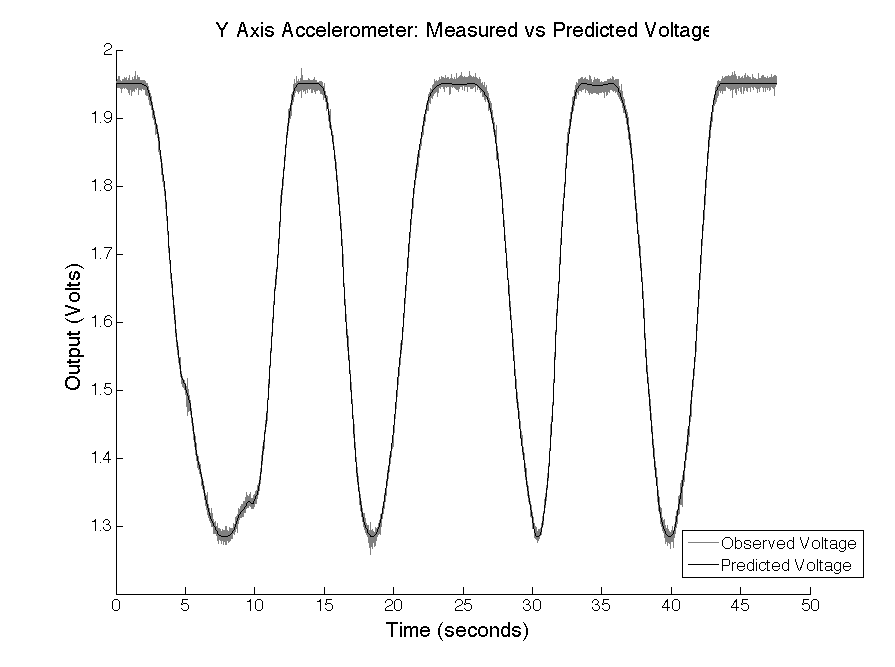
\includegraphics[width = 13cm]{YaxisAccel_Calib.png}
\caption{Expected vs Measured Voltages for the Y axis accelerometer}
\label{YaccelCalib}
\end{center}
\end{figure}

\begin{figure}
\begin{center}
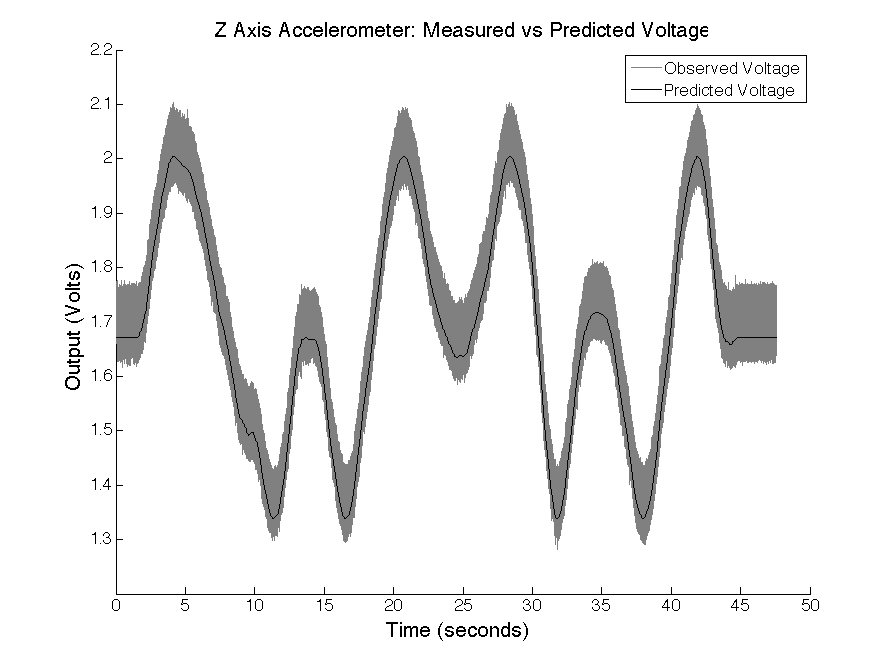
\includegraphics[width = 13cm]{ZaxisAccel_Calib.png}
\caption{Expected vs Measured Voltages for the Z axis accelerometer}
\label{ZaccelCalib}
\end{center}
\end{figure}

\subsection*{Rate Gyro}

% note that these calibration results were obtained from the natural frequency with the normal pendulum

A rate gyro outputs a voltage proportional to the angular rate about the sensitive axis of the gyro with some offset, the Zero Rate which is not ratiometric.  

$$V_{out} = ZeroRate + \Sens_{Gyro} \dot{\theta} $$

However even for a time period of a few seconds, we encountered several difficulties in trying to apply such a model.  First of all, the rate gyro's response is limited to higher frequencies requiring us to use an oscillating calibration run at the natural frequency of our pendulum sensor set up, of approximately 1.41 Hz.  The data was trimmed to only include the region of the response of a high enough frequency to be within the bandwidth of the sensor.  Secondly, even over this shorter calibration run, the Zero Rate was not constant.  To overcome these difficulties, we fit a slightly more complex model to obtain a good value for the sensitivity.

$$V_{out} = A t + B + \Sens_{Gyro} \dot{\theta} $$

Both $A$ and $B$ vary with time and other variables, such as temperature, so $B$, the zero rate of the gyro is determined on-line and A is neglected, so their values for this particular run are irrelevant.  

Assuming that the bandwidth of the DAQ and sensor system is 140 $(Hz)$ as described in the data sheet.  Noise density was computed from the total RMS noise value in the data sheet using the previously given formula, which was also then used to compute the expected noise over the lower bandwidth.

\begin{table}
\begin{center}
	\begin{tabular}{|c|c|}
		\hline
		
		$\Sens_{Gyro} \, \left( \sfrac{V s}{rad} \right)$ & 0.36 \\ 
		Total RMS Noise $(mV \, rms)$ & 0.8 \\ 
		Noise Density $\left( \sfrac{V}{\sqrt{Hz}}\right)$ & 2.0 \e{-5} \\ 
		Bandwidth $(Hz)$ & 140 \\ 
		$\sigma^2 \, \left( V^2 \right)$ & 8.96 \e{-8} \\ 
		\hline
	\end{tabular}
\caption{Performance parameters for the IDG-500 obtained from the data sheet.  \emph{Note that Noise Density and $\sigma^2$ were derived from data sheet values.}}
\label{ParamID_DatasheetGyro}
\end{center}
\end{table}

% quoted sensitivity = 1 / 8.635380
\begin{table}
\begin{center}
    \begin{tabular}{|c|c|c|c|c|}
        \hline
        ~   & Natural Frequency 1 & Natural Frequency 2 & Manual 1 & Manual 2\\ \hline
	Data Set Frequency (Hz)  & 1.41  & 1.76 & 2.42 & 5.13\\
        $\Sens_{Gyro} \, \left( \sfrac{V s}{rad} \right)$  & 0.115803  & 0.11672 & 0.11358 & 0.114821\\
	$\sigma^2 \, \left( V^2 \right)$  & $3.773 \e{-6}$ & $4.1077\e{-6}$ & 4.7680 \e{-6} & 4.1615\e{-5}\\
	Fitting Error $(rad)$ &  $3.358 \e{-4}$ & $4.206 \e{-4}$ & 2.814 \e{-4} & 2.050 \e{-4}\\
        \hline
    \end{tabular}
\caption{Gyro Sensitivity at a variety of frequencies within the full scale range.}  
\label{ParamID_TGyro}
\end{center}
\end{table}





\begin{figure}
\begin{center}
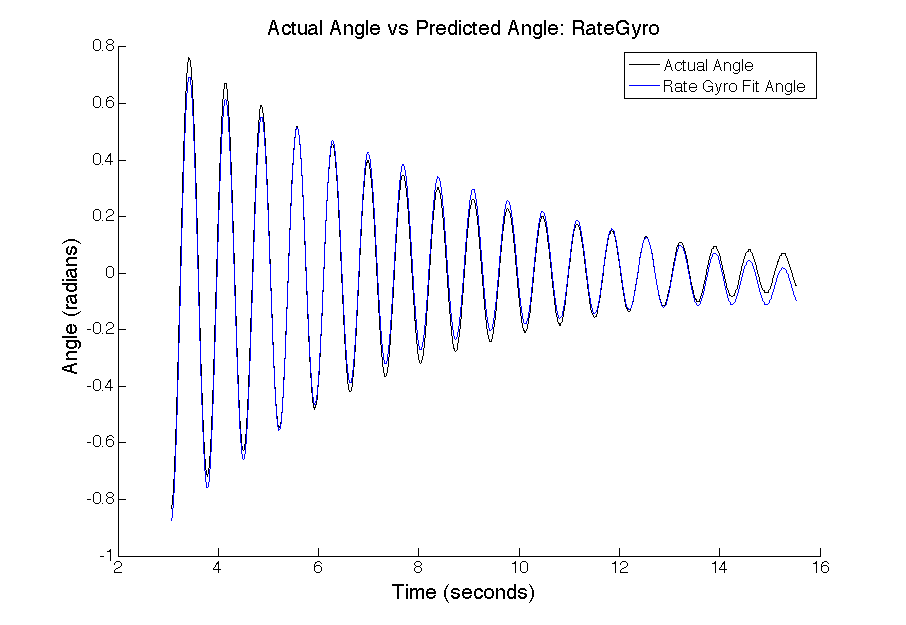
\includegraphics[width = 13cm]{rateGyroCalibResultsS8_636380.png}
\caption{Actual Angle vs Fitted Angle from integrating rate gyro output for Natural Frequency 1 trial}
\label{gyroCalib}
\end{center}
\end{figure}

\clearpage
\section{Low Frequency Characterization}

For all tests (in this low frequency section and all others), the Inertial Measurement Unit (IMU) breakout board was mounted as shown in figure \ref{sensorMount}. The IMU board was mounted on a small breadboard which was then attached to the side of the pendulum's shaft collar using double-sided tape. Mounting on the side was required to get the proper orientation to use one of the rate gyros. The flat face of the breadboard allowed us to minimize angular misalignment of the IMU. The position was arranged to minimize the distance of the sensor chips from the pendulum's axis of rotation. Washers were then attached to the opposite side of the shaft collar to counter-balance the breadboard, causing the pendulum to hang vertically. However, in some tests the stiffness of the wires caused a slight angular offset of the pendulum. Connections to one row of the IMU's pins were made through the breadboard, while the other row was accessed with female jumper wires.\\ 

Since the range of measurement for each sensing scheme was of interest, we made the pendulum slowly move in a full circle twice in both clockwise or counter clockwise directions. All angles were normalized into 0-360 deg region. For the resulting data, the angular velocity was assumed constant, so that its frequency was approximately equal to 0.05 Hz. To get cleaner measurements, three types of filters, (1) Kalman filter, (2) low-pass filter, and (3) moving-average filter, were tested. Figure~\ref{Filters_ZoomIn} shows the trajectory comparison of all filtering approaches. The low-pass filter and the moving average seem to have similar performance in terms of phase lag; thus, the low-pass filter was used for the following analyses due to its simplicity. Theroretically the upper limit of time constant could not exceed 0.5 considering the constraint of phase lag needed to be less than 10 deg. $\tau$ was initially set to 0.05.\\ 

\begin{figure}[hbt]
\begin{center}
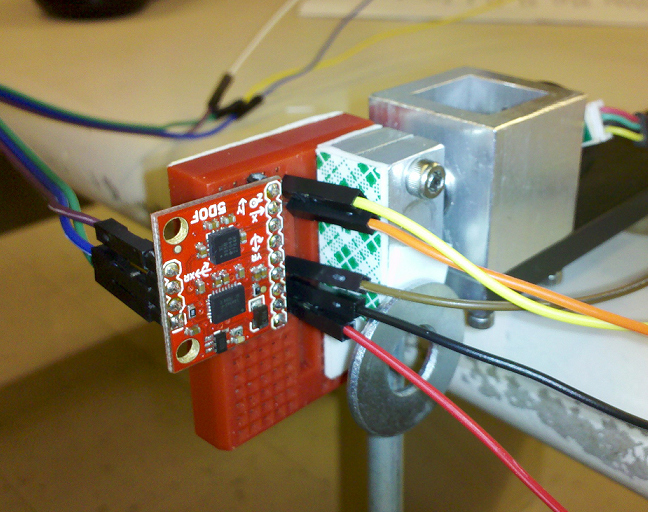
\includegraphics[width = 13cm]{SensorMounting.png}
\caption{Physical mounting of the IMU}
\label{sensorMount}
\end{center}
\end{figure}

\begin{figure}[hbt]
\begin{center}
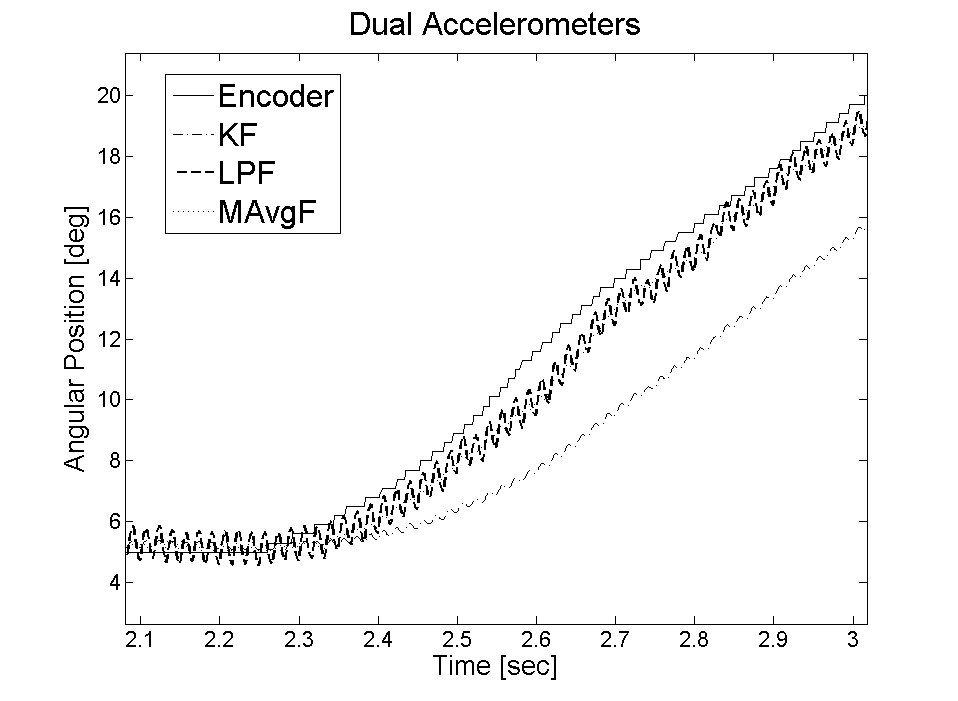
\includegraphics[width = 12cm]{Filters_ZoomIn.png}
\caption{Comparison of Filtering Approaches In Low-Frequency Region}
\label{Filters_ZoomIn}
\end{center}
\end{figure}

%%%%%%%%%%%%%%%%%%%%%%%%%%%%%%%%%%%%%%%%%%%%%%%%%%%%%%%%%
\subsection{Horizontal Accelerometer}

\subsubsection{Angle Measurement}

Using a single accelerometer in the horizontal configuration is equivalent to just using the Z axis in our configuration.  Where $V_{Z}$ is given as follows: 

$$ V_{Z}(\theta) = V_{Zbias} + \Sens_{Z} g \sin(\theta) $$

$\theta$ can be easily computed by the following expression:

\begin{equation}
\theta = \sin^{-1}\left( \frac{V_{Z} - V_{Zbias}}{\Sens_{Z} g}\right) 
\label{horizontalEQ}
\end{equation}

When using a single accelerometer in the horizontal configuration aliasing occurs for $|\theta| \geq \sfrac{\pi}{2}$.  It is important to note that the arcsine function has a restricted domain and is only valid on inputs between -1 and 1.  Noise and inaccurate estimates of the bias voltage, sensitivity and gravity can all drive the input quantity beyond this range.  To address this, we simply saturate inputs to restrict them to the valid range.

$$\theta = \left\{ 
	\begin{array}{l l}
		\sin^{-1} \left(\frac{V_{Z} - V_{Zbias}}{\Sens_{Z} g} \right) & {\bf{if }} \, \left| \frac{V_{Z} - V_{Zbias}}{\Sens_{Z} g} \right| \leq 1 \\[6pt]
		\frac{\pi}{2} & {\bf{if }} \, \frac{V_{Z} - V_{Zbias}}{\Sens_{Z} g} > 1 \\[6pt]
		-\frac{\pi}{2} & {\bf{if} } \, \frac{V_{Z} - V_{Zbias}}{\Sens_{Z} g} < -1
	\end{array} \right. $$

%%%%%%
Figure~\ref{Z_TimeDomain} shows the time domain plots from the optical encoder and the horizontal accelerometer. Figure~\ref{Z_ErrorPercentage} and Figure~\ref{Z_AbsError} show the percent errors and absolute errors with respect to angluar positions, respectively. Based on these results, the acceptable range of angular displacement is between $0^\circ$ - $63.8^\circ$, and $293.9^\circ$ - $360^\circ$. Compared to the theoretical values ( $0^\circ$ - $90^\circ$, and $270^\circ$ - $360^\circ$), the acutal range is smaller. It is reasonbale since the sensitivity at $90^\circ$ and $270^\circ$ goes to zero, and therefore the measurements around those regions are inaccurate. \\

\begin{figure}[hbt]
\begin{center}
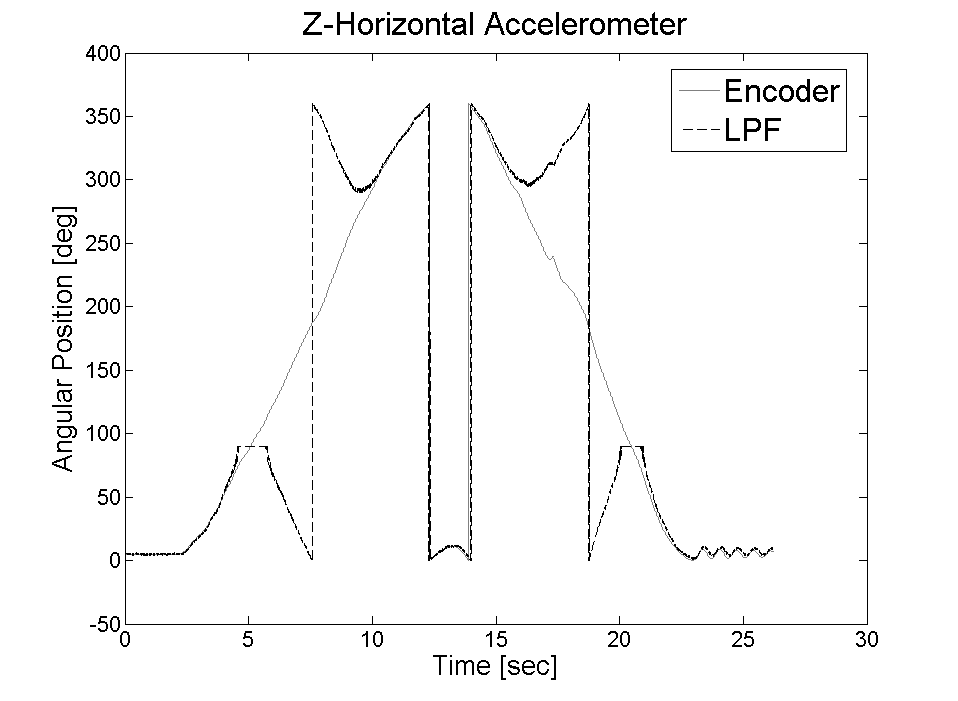
\includegraphics[width = 13cm]{Z_TimeDomain.png}
\caption{Angular Position vs. Time}
\label{Z_TimeDomain}
\end{center}
\end{figure}

\begin{figure}[hbt]
\begin{center}
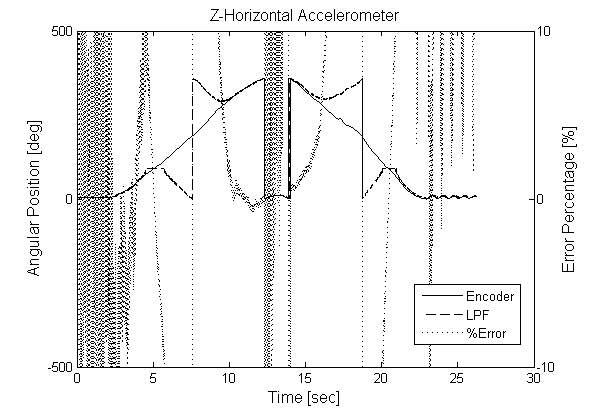
\includegraphics[width = 13cm]{Z_ErrorPercentage.png}
\caption{\% Error Percentage of Angular Position vs. Time}
\label{Z_ErrorPercentage}
\end{center}
\end{figure}

\begin{figure}[hbt]
\begin{center}
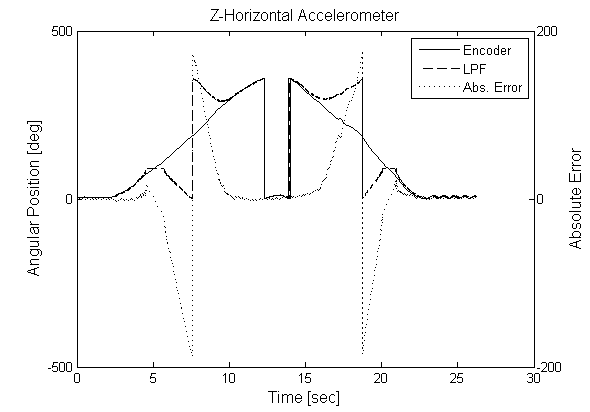
\includegraphics[width = 13cm]{Z_AbsError.png}
\caption{Absolute Error of Angular Position vs. Time}
\label{Z_AbsError}
\end{center}
\end{figure}
%%%%%%

\subsubsection{Sensitivity}

The relationship between sensor output voltage and angle is non-linear, but we are able to linearize about a particular operating point, for this experiment, $\theta = 0$, and obtain an estimate of the sensitivity.

$$ V_{Z}(\theta) \approx V_{Zbias} + \Sens_{Z} g \sin(0) + \Sens_{Z} g \cos(0) \left(\theta - 0\right) = V_{Zbias} + \Sens_{Z} g \theta $$

$$ \theta \approx \frac{V_{Z}(\theta) - V_{Zbias}}{S_Z g}  \quad \Sens_\theta \approx \frac{1}{\Sens_Z g}$$

For the horizontal accelerometer, we expect the sensitivity to be $\sfrac{1}{\Sens_{Z} g}$.  Figure~\ref{Z_Vol_vs_Angle} and Figure~\ref{Z_Sensibility} show the sensitivity and output voltages with respect to angular positions, respectively. It can be observed that the sensitivity function seems to be the derivative of arccosine function. The maximum is 5.82 mV at $0^\circ$ or $360^\circ$, and the sensitivity decreases to 0 when the measured angle closes to $90^\circ$ and $270^\circ$.

\begin{figure}[hbt]
\begin{center}
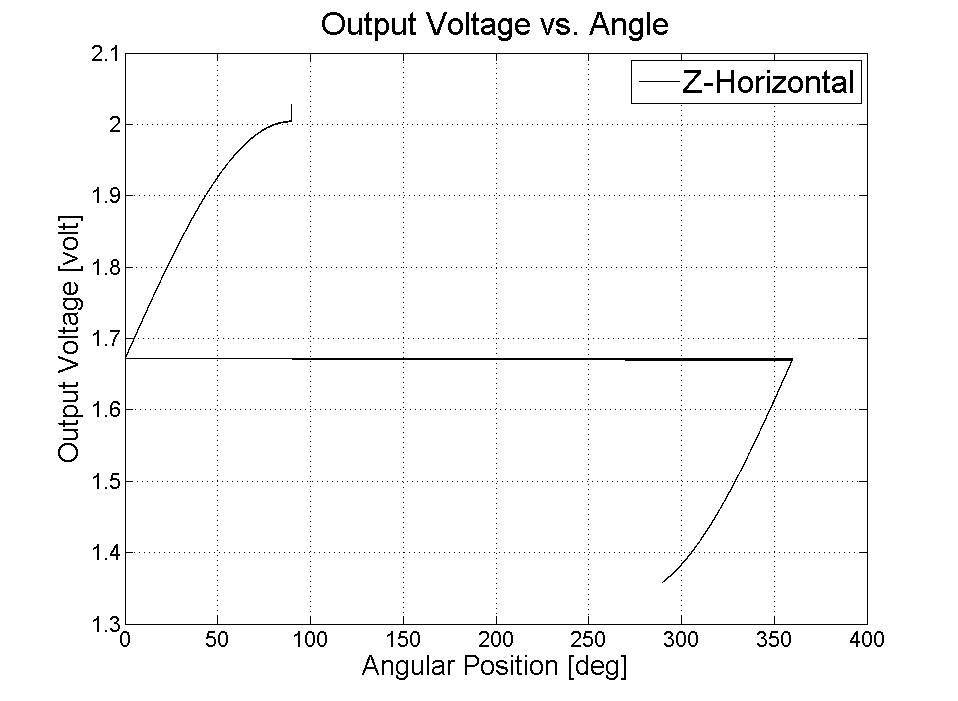
\includegraphics[width = 8.5cm]{Z_Vol_vs_Angle.png}
\caption{Z-Output Voltage vs. Angular Position}
\label{Z_Vol_vs_Angle}
\end{center}
\end{figure}

\begin{figure}[hbt]
\begin{center}
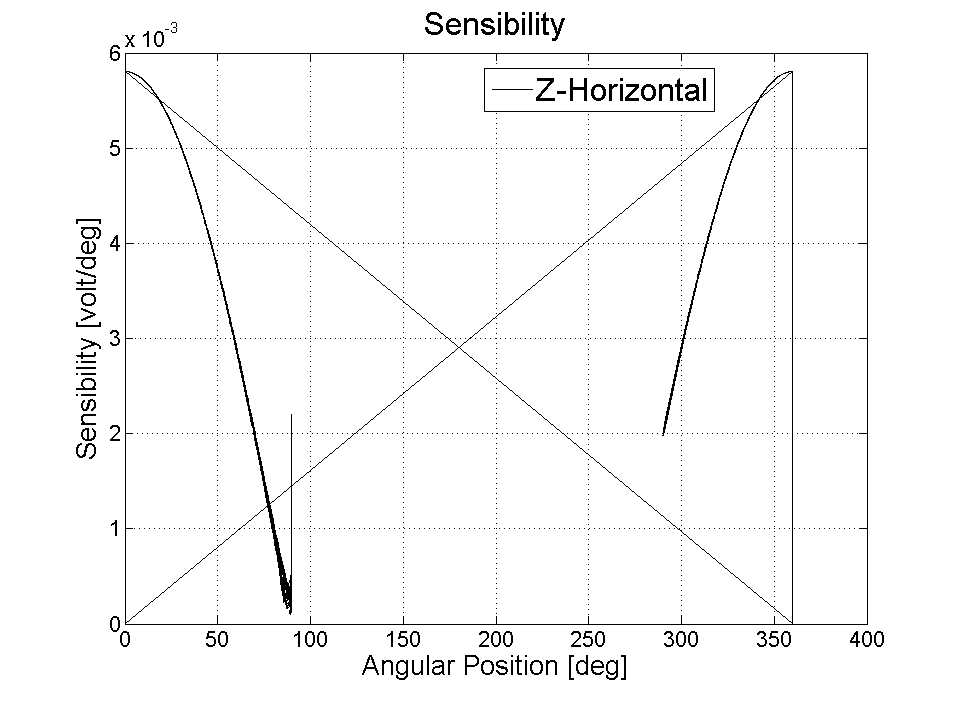
\includegraphics[width = 8.5cm]{Z_Sensibility.png}
\caption{Sensitivity vs. Angular Position}
\label{Z_Sensibility}
\end{center}
\end{figure}

\subsubsection{Noise}

An estimate for the expected noise in measurement of $\theta$ can be obtained by performing a variance projection through the partial derivative of equation \ref{horizontalEQ}.

$$ \frac{\partial \theta}{\partial V_{Z}} =  \frac{1}{\sqrt{(\Sens_{Z} g)^2 - (V_{Z} - V_{Zbias})^2}}$$

$$ \sigma^2_{\theta} = \frac{\partial \theta}{\partial V_{Z}} \sigma^2_{V_{Z}} \frac{\partial \theta}{\partial V_{Z}} $$

$$ \sigma^2_{\theta} = \frac{\sigma^2_{V_{Z}}}{(\Sens_{Z} g)^2 - (V_{Z} - V_{Zbias})^2}$$

For $\theta \approx 0$ we would expect the noise of our angle measurements to be given by:

$$ \theta \approx 0 \quad \sigma^2_{\theta} \approx \frac{\sigma^2_{V_{Z}}}{(\Sens_{Z} g)^2}$$

The following data was collected for a fixed vertical pendulum, $\alpha = 0$.  It seems that there was a discrepancy betweeen the earlier recorded bias voltage for the Z-axis, and the bias voltage for this trial.  Besides that difference, the mean and variance very closely resemble the expected values, but as noted earlier the noise is significantly worse than promised by the data sheet.  

% comparison to real data here
\begin{table}
\begin{center}
    \begin{tabular}{|c|c|c|}
        \hline
        ~                   & Theoretical  & Actual \\ \hline
        $\sigma^2_{V_{Z}} \, (V^2)$    & 0.001852504            &  0.00185231      \\ 
        $\sigma^2_{\theta} \, (rad^2)$ & 0.01674716            & 0.0169008      \\ 
        $\mu_{V_{Z}} \, (V)$       & 1.671451851            &  1.701057      \\ 
        $\mu_{\theta} \, (rad)$      & 0            &  -1.219912 \e{-5}     \\
        Peak to Peak $(V)$ & ~ & 0.143 \\
        Peak to Peak $(rad)$ & ~ & 0.4528 \\
        \hline
    \end{tabular}
\caption{Comparison of theoretical noise in $\theta$ with measured noise in $\theta$ for the horizontal accelerometer alone. \emph{Note that the theoretical variance of voltage and bias were measured in another trial.}}
\label{Noise_horizontal_T}
\end{center}
\end{table}

Figure~\ref{Z_Peak2peak} shows the real behavior of fluctuation based on a fixed angle. The peak to peak noise level is approximately 1.83$^{\circ}$.

\begin{figure}[hbt]
\begin{center}
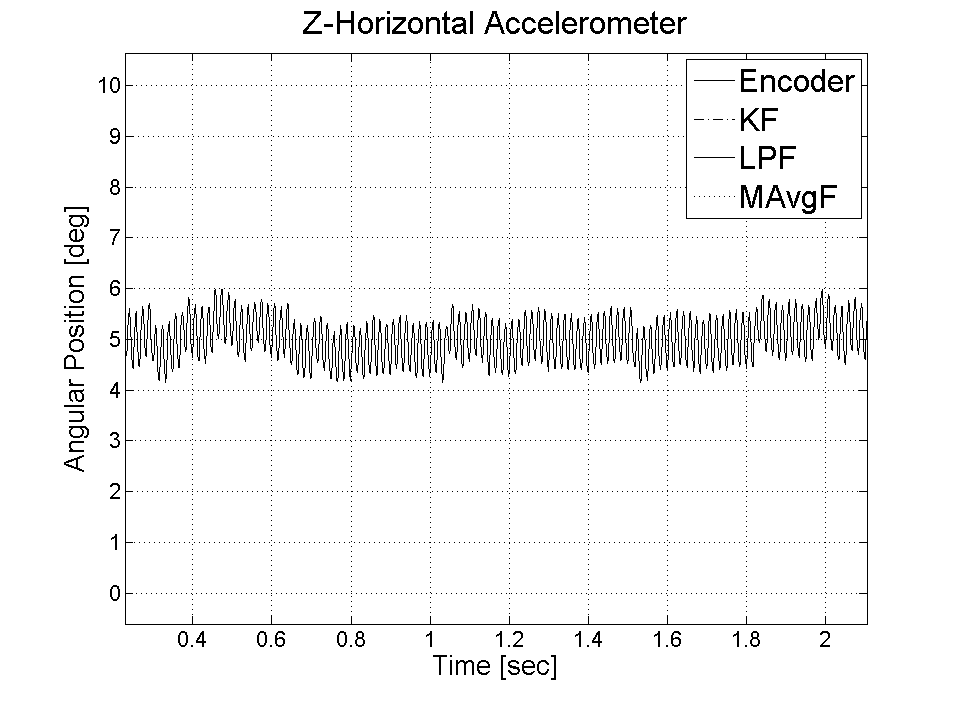
\includegraphics[width = 13cm]{Z_Peak2peak.png}
\caption{Angular Position vs. Time}
\label{Z_Peak2peak}
\end{center}
\end{figure}

%%%%%%%%%%%%%%%%%%%%%%%%%%%%%%%%%%%%%%%%%%%%%%%%%%%%%%%%%
\subsection{Vertical Accelerometer}

\subsubsection{Angle Measurement}

Using a single accelerometer in the vertical configuration is equivalent to using just the Y axis in our configuration.  Where $V_{Y}$ is given as follows:

$$ V_{Y} = V_{Ybias} + \Sens_{Y} g \cos(\theta) $$

Then $\theta$ is given by the following expression:

\begin{equation}
\theta = \cos^{-1}\left( \frac{V_{Y} - V_{Ybias}}{\Sens_{Y} g}\right)
\label{verticalEQ}
\end{equation}

When using a single accelerometer in this configuration aliasing occurs for angles beyond the range $0 \leq \theta \leq \pi$.  This range is much less useful than the range for a single accelerometer in the horizontal configuration because we are unable to read negative angles immediately next to our starting condition, $\theta = 0$.  The arccosine function also has a limited domain, from 1 to -1, and we simply limit it to the valid range as in the horizontal accelerometer case above.

$$\theta = \left\{ 
	\begin{array}{l l}
		\cos^{-1}\left( \frac{V_{Y} - V_{Ybias}}{\Sens_{Y} g}\right) & {\bf{if }} \, \left| \frac{V_{Y} - V_{Ybias}}{\Sens_{Y} g} \right| \leq 1 \\[6pt]
		0 & {\bf{if }} \, \frac{V_{Y} - V_{Ybias}}{\Sens_{Y} g} > 1 \\[6pt]
		-\pi & {\bf{if} } \, \frac{V_{Y} - V_{Ybias}}{\Sens_{Y} g} < -1
	\end{array} \right. $$


Figure~\ref{Y_TimeDomain} shows the time domain plots from the optical encoder and the horizontal accelerometer. Figure~\ref{Y_ErrorPercentage} and Figure~\ref{Y_AbsError} show the percent errors and absolute errors with respect to angluar positions, respectively. Based on these results, the acceptable range of angular displacement is between $54.8^\circ$ - $194^\circ$ (1st circle), or $183^\circ$ - $24.25^\circ$ (2nd circle). Compared to the theoretical values ( $0^\circ$ - $180^\circ$), the actual range is smaller as expected since the sensitivity at $0^\circ$ and $180^\circ$ goes to zero; thus, the measurements near that region are inaccurate. Although the error around $180^\circ$ seems acceptable, the measured angles from the accelerometer are saturated at $180^\circ$. \\

\begin{figure}[hbt]
\begin{center}
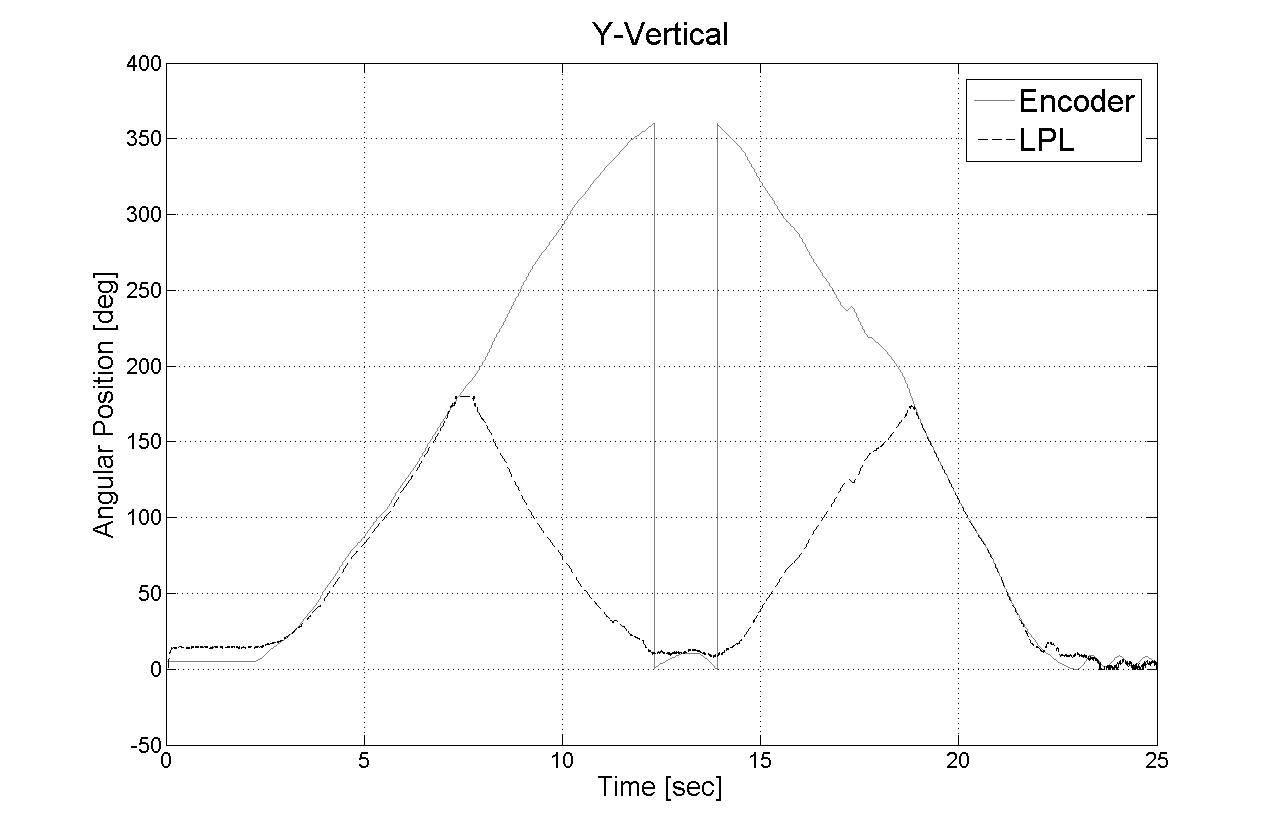
\includegraphics[width = 12cm]{Y_TimeDomain.png}
\caption{Angular Position vs. Time}
\label{Y_TimeDomain}
\end{center}
\end{figure}

\begin{figure}[hbt]
\begin{center}
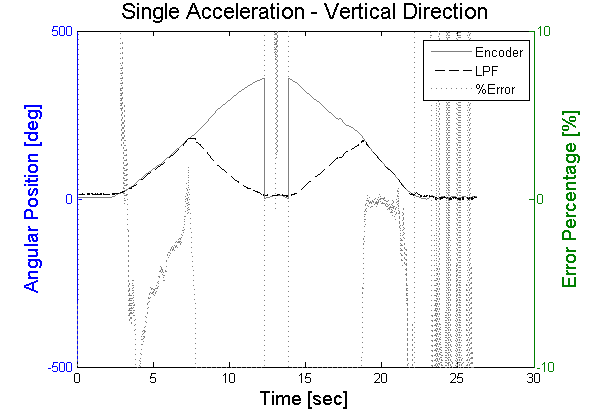
\includegraphics[width = 13cm]{Y_ErrorPercentage.png}
\caption{\%Error Percentage of Angular Position vs. Time}
\label{Y_ErrorPercentage}
\end{center}
\end{figure}

\begin{figure}[hbt]
\begin{center}
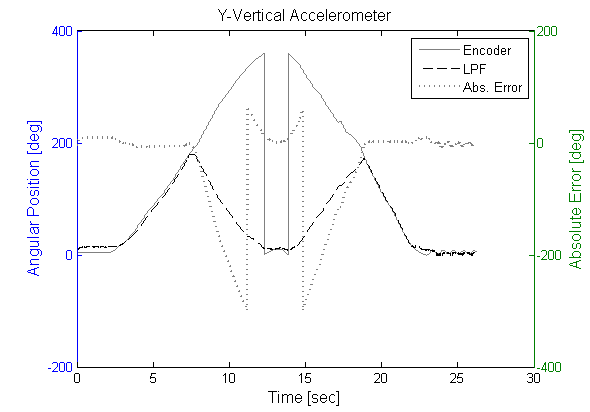
\includegraphics[width = 13cm]{Y_AbsError.png}
\caption{Absolute Error of Angular Position vs. Time}
\label{Y_AbsError}
\end{center}
\end{figure}

\subsubsection{Sensitivity}

However linearizing about $\theta = 0$ for the accelerometer in the vertical configuration is not particularly successful,  yielding a relationship that does not depend on $\theta$ at all.  This result is expected from our earlier assessment of the angle ambiguity between positive values of $\theta$ and negative values.  

$$V_{Y}(\theta) \approx V_{Ybias} + \Sens_{Y} g \cos(0) - \Sens_{Y} g \sin(0) (\theta - 0) = V_{Ybias} + \Sens_{Y} g $$

$$ \Sens_\theta \approx 0 $$

In this case the output voltage of the sensor does not depend on the angle $\theta$ so we have effectively 0 sensitivity. Figure~\ref{Y_Vol_vs_Angle} and Figure~\ref{Y_Sensibility} show the sensitivity and output voltages with respect to angular positions, respectively. It can be observed that the sensitivity function seems to be the derivative of arcsine function. The maximum is 5.80 mV at $90^\circ$, and the sensitivity decreases to 0 when the measured angle closes to $0^\circ$ or $180^\circ$.

\begin{figure}[hbt]
\begin{center}
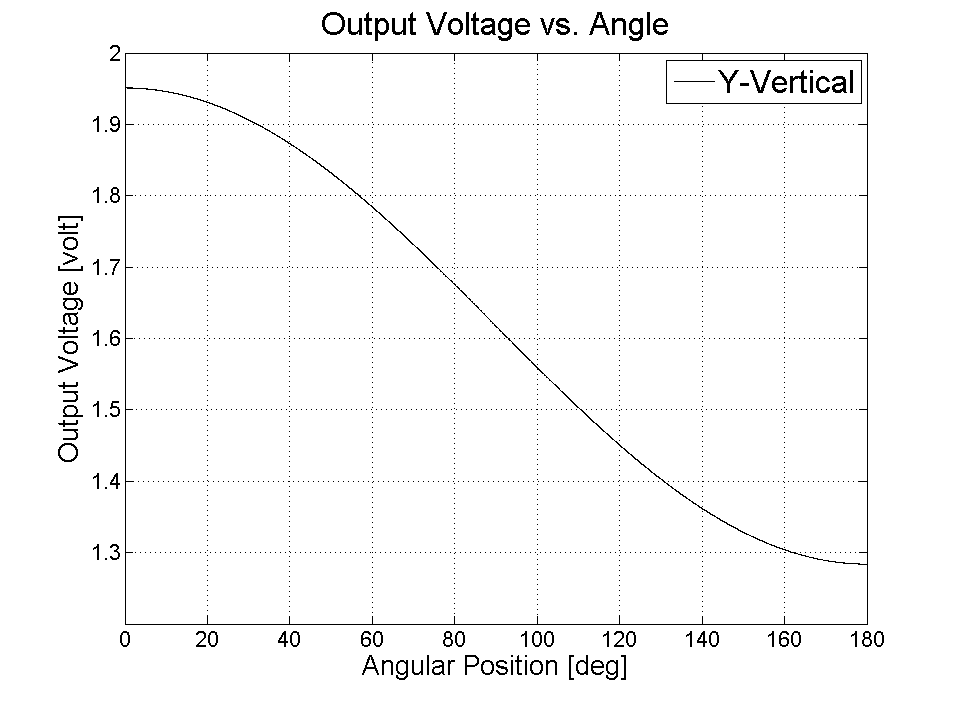
\includegraphics[width = 10cm]{Y_Vol_vs_Angle.png}
\caption{Y-Output Voltage vs. Angular Position}
\label{Y_Vol_vs_Angle}
\end{center}
\end{figure}

\begin{figure}[hbt]
\begin{center}
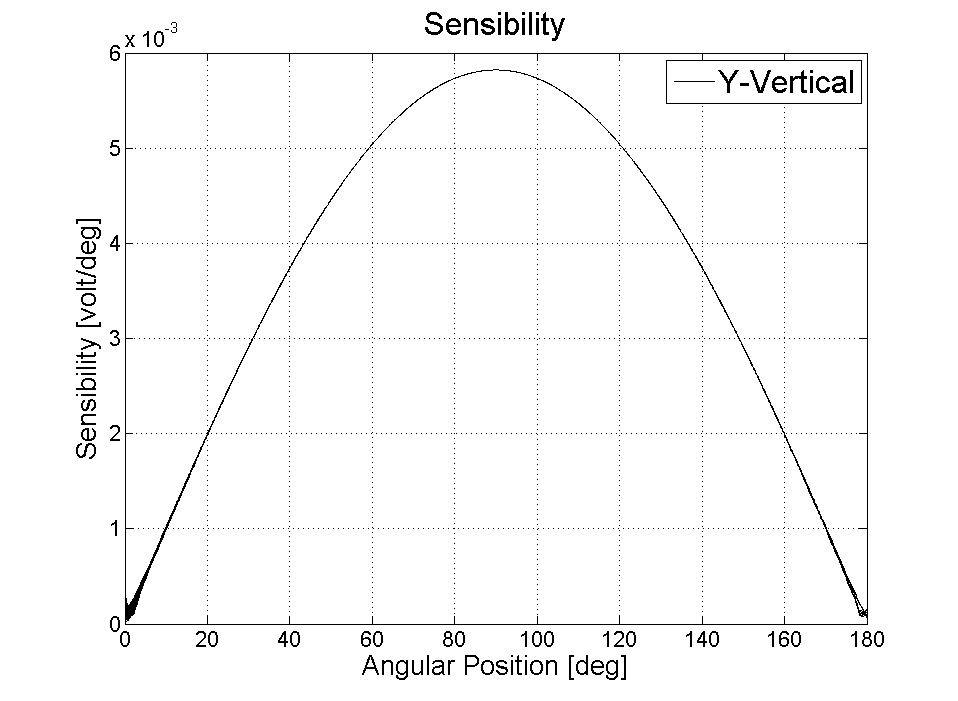
\includegraphics[width = 10cm]{Y_Sensibility.png}
\caption{Sensitivity vs. Angular Position}
\label{Y_Sensibility}
\end{center}
\end{figure}

\subsubsection{Noise}

As before, the following noise trial was conducted for a fixed vertical pendulum, with $\alpha = 0$. We can again use variance projection to estimate the noise in our angle measurements, taking the partial derivative of equation \ref{verticalEQ}.

$$ \frac{\partial \theta}{\partial V_{Y}} = -\frac{1}{\sqrt{(\Sens_{Y} g)^2 - (V_{Y} - V_{Ybias})^2}}$$

$$ \sigma^2_{\theta} = \frac{\partial \theta}{\partial V_{Y}} \sigma^2_{V_{Y}} \frac{\partial \theta}{\partial V_{Y}} $$

$$ \sigma^2_{\theta} = \frac{\sigma^2_{V_{Y}}}{(\Sens_{Y} g)^2 - (V_{Y} - V_{Ybias})^2}$$

As we would expect, this appears identical to the equation for noise of the horizontally mounted accelerometer.  The difference in behavior is simply the voltage around which we linearize.  Substituting the value for $V_{Y}$ about $\theta = 0$  yields a surprising result.

% is this result just a quirk of the linearization?

$$ \theta \approx 0 \quad \sigma^2_{\theta} \approx \frac{\sigma^2_{V_{Y}}}{(\Sens_{Y} g)^2 - (V_{Ybias} + \Sens_{Y} g - V_{Ybias})^2} = \infty$$

What has happened, is that the above calculation neglected the effects of our earlier signal conditioning.  While the expected voltage is $V_{Ybias} + \Sens_Y g$.  The expected value of the quantity within the arccosine is not 1.  Because of the saturation conditioning used to prevent arccosine from failing, the actual distribution is no longer Gaussian, and most importantly is not symmetric about 0 which leads to the relatively large deviation from the expected mean of desired mean of 0.  Analytially calculating the mean and variance of this distribution would be troublesome, so rather than use the variance projection techniques utilized earlier, we instead used a simple numerical technique.  We drew samples of the sensor voltage in the vertical configuration using our estimates of the Y-axis sensor bias voltage, the voltage noise, sensitivity, and acceleration due to gravity.  Then we applied our signal conditioning technique, and calculated $\theta$ from these samples, and with these samples of $\theta$ estimated their mean and variance, shown in table \ref{Noise_vertical_T}.  The matlab code utilized is shown in the appendix.s\\

%$$ E \left[ \frac{V_{Y} - V_{Ybias}}{\Sens_{Y} g} \right] \approx 0.5 \cdot 1 + 0.5 \cdot \big(1 - \sigma_{V_Y} \sqrt{\sfrac{2}{\pi}} \big) = 0.99859205 $$

%$$ E\left[ \cos^{-1} \left(  E \left[ \frac{V_{Y} - V_{Ybias}}{\Sens_{Y} g} \right]  \right)  \right] = 0.0530713 \, (rad) $$

%The variance of this sort of distribution is given by: 

% think I'm a bit off in this calculation, I didn't quite take into account the fact that it isn't just a half gaussian, we've got that spike at 1, http://en.wikipedia.org/wiki/Half-normal_distribution
% what I have is a clipped normal distribution
%\xxx{verify this one calculation, it seems a little bit off - - - - - - -   V}
%$$ \sigma_{arg1}^2 = \frac{\sigma^2_{V_Y}}{(\Sens_Y g)^2} = 1.11939534 \e{-4} \quad \sigma_{arg2}^2 = \sigma_{arg}^2 \left(1 - \frac{2}{\pi} \right) = 4.06766136 \e{-5}$$

%Then all that is left to do is to linearize the arccosine about this new mean:

%$$ \frac{d}{dx} \cos^-1(0.99859205) = -\frac{1}{\sqrt{1 - 0.99859205^2}} = -18.85143028 $$

%\emph{Because the function is highly nonlinear in this region, the variance estimate is not going to be particularly accurate.}  

%Finally the variance can be obtained:

%$$ \sigma_{\theta}^2 = \left( \frac{d}{dx} \cos^-1(0.99859205) \right) ^2 \sigma_{arg2}^2 = 0.01445551 $$

% comparison to real data here
\begin{table}
\begin{center}
    \begin{tabular}{|c|c|c|}
        \hline
        ~                   & Theoretical  & Actual \\ \hline
        $\sigma^2_{V_{Y}} \, (V^2)$    & 1.24553\e{-5}  & 5.807739 \e{-5}      \\ 
	$\sigma^2_{\theta} \, (rad^2)$ &  0.004875171          &  0.009754764     \\ 
	$\mu_{V_{Y}} \, (V)$       & 1.95100270            & 1.95268     \\
        $\mu_{\theta} \, (rad)$      & 0.05982302            & 0.09371065      \\
        Peak to Peak Noise (V) & ~  & 0.042 \\
        Peak to Peak Noise (rad) & ~ & 0.354 \\
        \hline
    \end{tabular}
\caption{Comparison of theoretical noise in $\theta$ with measured noise in $\theta$ for the Y axis accelerometer alone. \emph{Note that the theoretical variance of voltage and expectation was calculated from sensitivity and bias voltage measured in another trial.}  Noise values are for unfiltered data.}
\label{Noise_vertical_T}
\end{center}
\end{table}

This experiment verifies our suspicions that the mean would not be 0, and the estimated mean and variance were quite similar to the observed values, and the difference between them can largely be attributed to the difference in variance measured in trial run, and the variance in this particular trial. \\

Figure ~\ref{Y_Peak2peak} shows the real behavior of fluctuation based on a fixed angle. The peak to peak noise level is approximately 1.29$^{\circ}$.\\

\begin{figure}[hbt]
\begin{center}
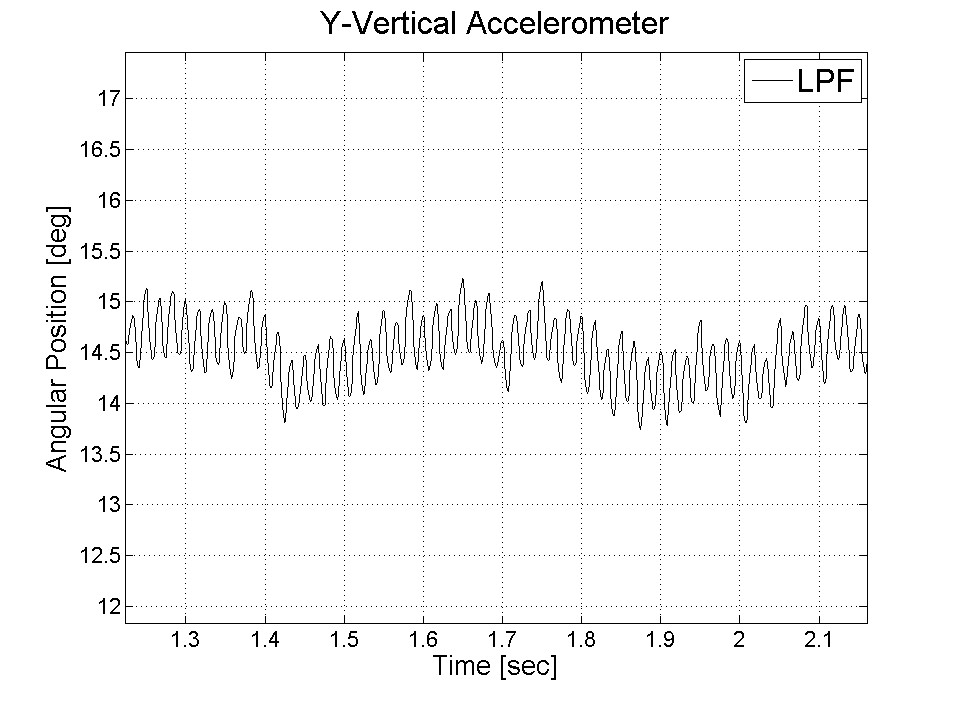
\includegraphics[width = 13cm]{Y_Peak2peak.png}
\caption{Angular Position vs. Time}
\label{Y_Peak2peak}
\end{center}
\end{figure}

%%%%%%%%%%%%%%%%%%%%%%%%%%%%%%%%%%%%%%%%%%%%%%%%%%%%%%%%%
\subsection{Two Accelerometers}

\subsubsection{Angle Measurement}

We can overcome the aliasing issue  presented in the two previous configurations by using both the horizontal and vertical, the Z and Y axis, simultaneously.  

$$ \cos(\theta) = \frac{V_Y-V_{Ybias}}{\Sens_{Y} g} \quad \sin(\theta) = \frac{V_{Z} - V_{Zbias}}{\Sens_{Z} g} $$

Combining the two equations gives the following:

$$ \tan(\theta) = \frac{\sin(\theta)}{\cos(\theta)} = \left(\frac{V_{Z} - V_{Zbias}}{\Sens_{Z} g}\right) \left( \frac{\Sens_{Y} g}{V_Y-V_{Ybias}} \right) = \frac{\Sens_{Y}}{\Sens_{Z}} \left( \frac{V_{Z} - V_{Zbias}}{V_{Y} - V_{Ybias}} \right)$$

Using the atan2 function avoids the quadrant ambiguities present in the ordinary $\tan^{-1}$ function giving us an expression for $\theta$ valid for all angles.

$$\theta = \text{atan2}\big( \Sens_{Y} \left( V_{Z} - V_{Zbias}\right),  \Sens_{Z} \left( V_{Y} - V_{Ybias}\right) \big)$$

Figure~\ref{Dual_TimeDomain} shows the time domain plots from the optical encoder and the dual accelerometers. Figure~\ref{Dual_ErrorPercentage} and Figure~\ref{Dual_AbsError} show the percent errors and absolute errors with respect to angluar positions, respectively. Based on these results, the acceptable range of angular displacement is between $0^\circ$ - $360^\circ$ (1st circle), or $360^\circ$ - $0^\circ$ (2nd circle). The theoretical values ( $0^\circ$ - $360^\circ$) and the actual range are almost identical, and the measurement of a full circle can be achieved. 

\begin{figure}[hbt]
\begin{center}
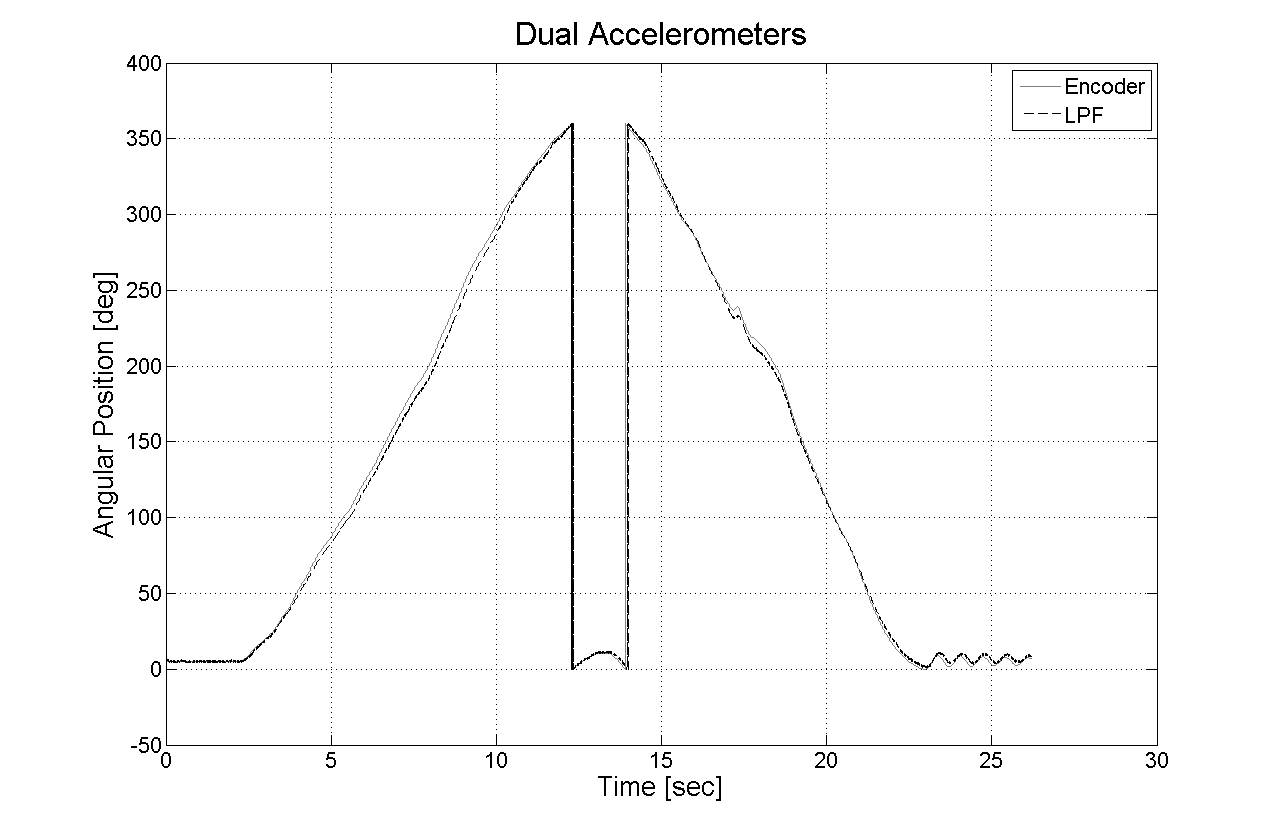
\includegraphics[width = 13cm]{Dual_TimeDomain.png}
\caption{Angular Position vs. Time}
\label{Dual_TimeDomain}
\end{center}
\end{figure}

\begin{figure}[hbt]
\begin{center}
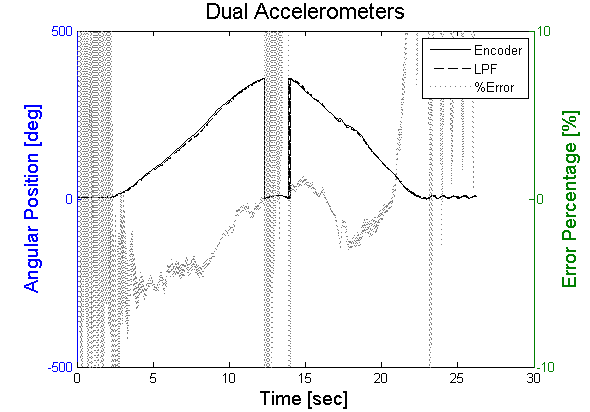
\includegraphics[width = 13cm]{Dual_ErrorPercentage.png}
\caption{\% Error Percentage of Angular Position vs. Time}
\label{Dual_ErrorPercentage}
\end{center}
\end{figure}

\begin{figure}[hbt]
\begin{center}
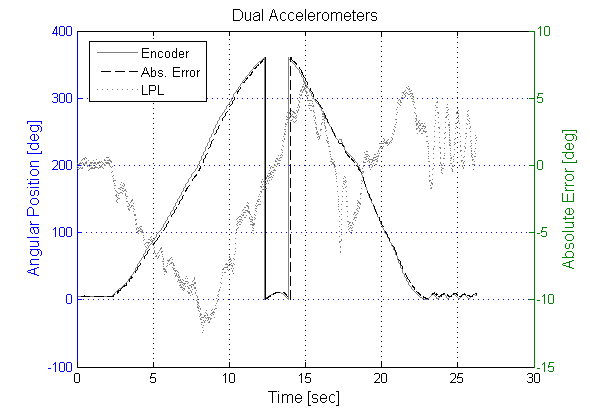
\includegraphics[width = 13cm]{Dual_AbsError.png}
\caption{Absolute Error of Angular Position vs. Time}
\label{Dual_AbsError}
\end{center}
\end{figure}

\clearpage
\subsubsection{Sensitivity}

Sensitivity of our angle measurement, $\theta$ is simply given by the partial derivatives, shown in equations \ref{dualAccel_partialVY} and \ref{dualAccel_partialVZ} of our expression for $\theta$ shown in equation \ref{dualAccel_EQ}.

\begin{equation}
\theta = \tan^{-1} \left( \frac{\Sens_{Y} \left( V_{Z} - V_{Zbias}\right)}{\Sens_{Z} \left( V_{Y} - V_{Ybias}\right)} \right) = f(V_{Y},V_{Z}) \approx f(V_{Y0},V_{Z0}) + \frac{\partial f}{\partial V_{Y}} \left( V_Y - V_{Y0} \right) + \frac{\partial f}{\partial V_Z} \left( V_Z - V_{Z0}\right)  
\label{dualAccel_EQ}
\end{equation}

\begin{equation}
\frac{\partial f}{\partial V_{Y}} = \frac{\Sens_Z \Sens_Y \left(V_{Z} - V_{Zbias} \right)}{\Sens^2_Y \left(V_Z - V_{Zbias} \right) ^2 + \Sens^2_Z \left( V_Y - V_{Ybias}\right)^2}
\label{dualAccel_partialVY}
\end{equation}

\begin{equation}
\frac{\partial f }{\partial V_Z} = \frac{\Sens_Z \Sens_Y \left(V_{Y} - V_{Ybias} \right)}{\Sens^2_Y \left(V_Z - V_{Zbias} \right) ^2 + \Sens^2_Z \left( V_Y - V_{Ybias}\right)^2}
\label{dualAccel_partialVZ}
\end{equation}

For $\theta \approx 0$, the sensitivity to the Y axis drops to 0 and the sensitivity to the Z axis is given by the same expression as before. 
Yielding the same sensitivity as the horizontal accelerometer alone.

$$ V_{Z0} = V_{Zbias}  \quad  V_{Y0} = V_{Ybias} + \Sens_{Y} g  \quad \frac{\partial f}{\partial V_{Y}} \approx 0  \quad \frac{\partial f }{\partial V_Z} = \frac{1}{\Sens_{Z} g}$$

$$ \theta \approx \frac{V_{Z}(\theta) - V_{Zbias}}{S_Z g}  \quad \Sens_\theta \approx \frac{1}{\Sens_Z g}$$

Figure~\ref{Dual_Sensibility} plots the sensitivity when the angular displacement changes. The result is simply the combination of both horizontal and vertical sensitivity functions. 

\begin{figure}[hbt]
\begin{center}
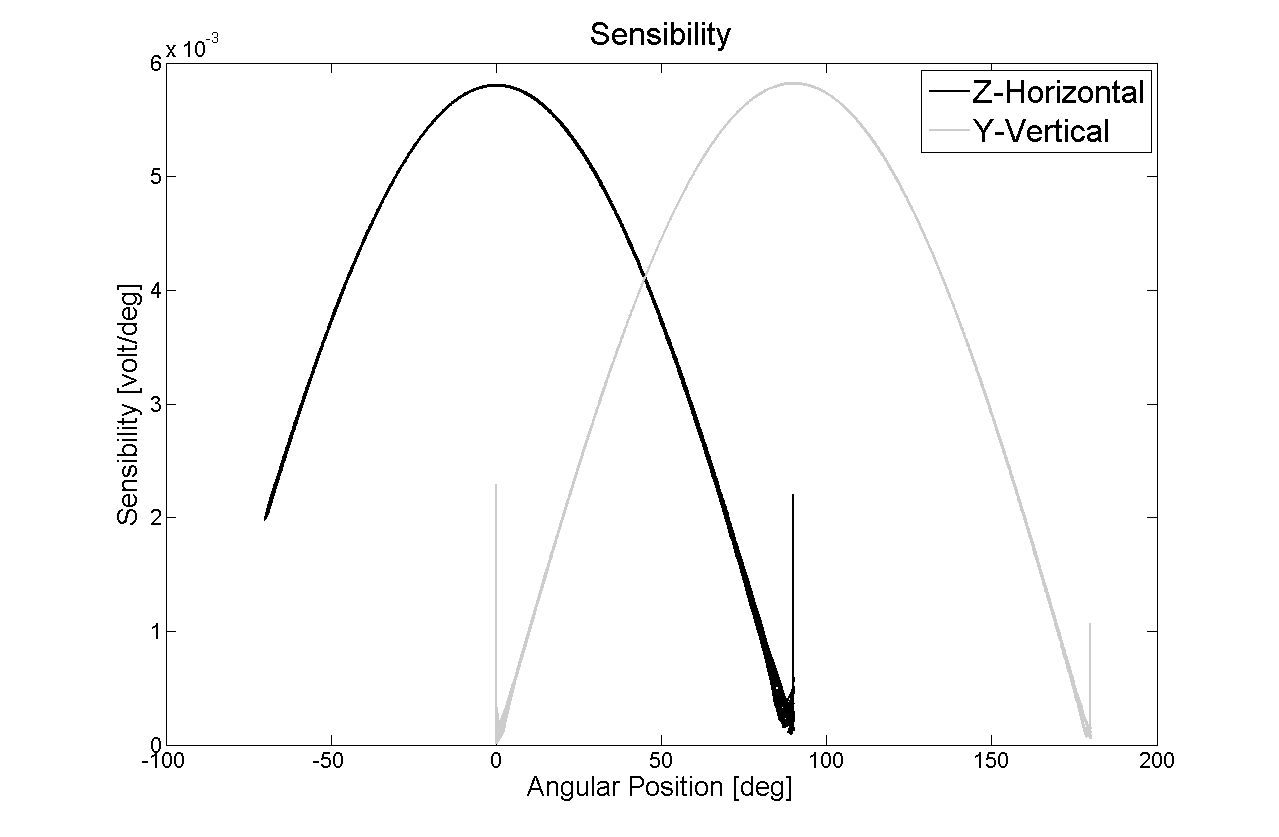
\includegraphics[width = 13cm]{Dual_Sensibility.png}
\caption{Sensitivity vs. Angular Position}
\label{Dual_Sensibility}
\end{center}
\end{figure}

\clearpage
\subsubsection{Noise}

Determining the expected noise is a bit more complicated for functions of several variables and requires a bit more math, shown below.   

Let 

$$ \vec{x} = \left[ V_Y, V_Z \right]^T $$

Then

$$ \theta = f(\vec{x}) \approx J|_{\vec{x}_0} \left( \vec{x} - \vec{x}_{0}\right) \quad J = \left[ \frac{\partial f}{\partial V_{Y}}, \frac{\partial f }{\partial V_Z} \right] $$

$$ \sigma^2_{\theta} = \Sigma_{\theta} = J \Sigma_{\vec{x}} J^T  \quad 
\Sigma_{\vec{x}} = \left[
\begin{matrix}
\sigma^2_{V_{Y}}  & 0 \\
0 & \sigma^2_{V_{Z}} 
\end{matrix} \right]$$

$$ \sigma^2_{\theta} = \left(\frac{\partial f}{\partial V_{Y}}\right)^2 \sigma^2_{V_{Y}} + \left(\frac{\partial f }{\partial V_Z} \right)^2 \sigma^2_{V_{Z}} $$

For our trial conducted with the pendulum in the vertical position, $\alpha = 0$, we can simply plug in $\theta = 0$ into our earlier equations to estimate the noise in this angle measurement.  For $\theta = 0$, the noise is approximately equal to the noise using only the horizontal axis of the accelerometer, which turns out ot be almost exactly true, though the variance does not quite match the actual value considering just the horizontal axis.

$$ \theta \approx 0 \quad V_{Z}(\theta) \approx V_{Zbias} + \Sens_{Z} g \theta \quad V_{Y}(\theta)  \approx V_{Ybias} + \Sens_{Y} g $$

$$ \frac{\partial f}{\partial V_{Y}} \approx 0  \quad \frac{\partial f }{\partial V_Z} = \frac{1}{\Sens_{Z} g}$$

$$ \sigma^2_{\theta} \approx \left(0\right)^2 \sigma^2_{V_{Y}} + \left(\frac{1}{\Sens_{Z} g} \right)^2 \sigma^2_{V_{Z}} = \left( \frac{\sigma_{V_Z}}{\Sens_{Z} g} \right)^2$$

% comparison to real system
\begin{table}
\begin{center}
    \begin{tabular}{|c|c|c|}
        \hline
        ~                   & Theoretical  & Actual \\ \hline
        $\sigma^2_{V_{Z}} \, (V^2)$    & 0.001852504            & 0.001852312     \\ 
	$\mu_{V_{Z}} \, (V)$       & 1.671451851            & 1.7010571      \\ 
	$\sigma^2_{V_{Y}} \, (V^2)$ & 1.24553\e{-5}		& 5.8077389 \e{-5} \\
	$\mu_{V_{Y}} \, (V)$       & 1.95100270            & 1.619099      \\ 
        $\sigma^2_{\theta} \, (rad^2)$ & 0.01674716             &  0.01647518     \\ 
        $\mu_{\theta} \, (rad)$      & 0            & -0.002390427      \\
        Peak to Peak $V_Z \, (V)$ &  ~ & 0.143 \\
        Peak to Peak $V_Y \, (V)$ & ~  & 0.042 \\
        Peak to Peak $(rad)$ & ~ & 0.4443 \\
        \hline
    \end{tabular}
\caption{Comparison of expected noise and actual noise for $\theta = 0$ using both accelerometer axes.  Noise for unfiltered data.}
\label{Noise_dual_T}
\end{center}
\end{table}

Figure ~\ref{Dual_Peak2peak} shows the real behavior of fluctuation based on a fixed angle. The peak to peak noise level is approximately 1.84$^{\circ}$.

\begin{figure}[hbt]
\begin{center}
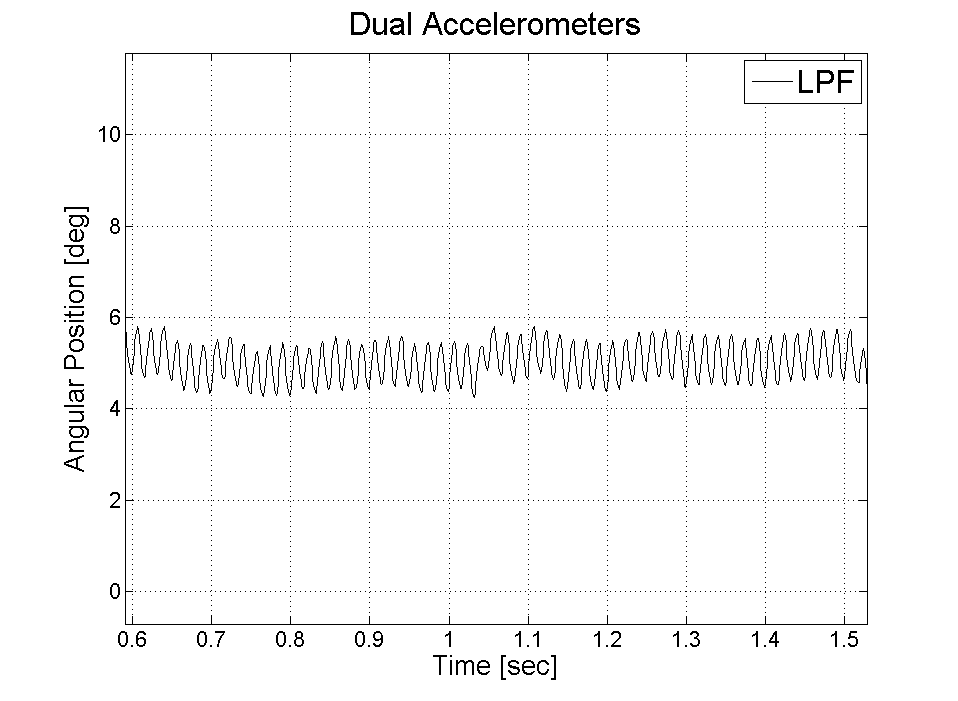
\includegraphics[width = 13cm]{Dual_Peak2peak.png}
\caption{Angular Position vs. Time}
\label{Dual_Peak2peak}
\end{center}
\end{figure}

%%%%%%%%%%%%%%%%%%%%%%%%%%%%%%%%%%%%%%%%%%%%%%%%%%%%%%%%%
\subsection{Rate Gyro}

\subsubsection{Angle Measurement}

As mentioned earlier, the output voltage of the rate gyro is assumed to be linearly related to the angular velocity about the sensitive axis of the gyro as shown in the equation repeated below.  The Zero Rate and the sensitivity of the gyro are assumed to be time invariant.  Solving for $\dot{\theta}$ yields:

$$V_{Gyro}(t) = ZeroRate_{Gyro} + \Sens_{Gyro} \dot{\theta}(t) $$

$$\dot{\theta}(t) = \frac{V_{Gyro}(t) - ZeroRate_{Gyro}}{\Sens_{Gyro}} $$

Integrating the expression for $\dot{\theta}$ yields $\theta$, and this integral is approximated by applying the trapezoid rule for numerical quadrature.

$$ \theta(t) = \int_0^t \dot{\theta}(\tau) d\tau = \int_0^t \frac{V_{Gyro}(\tau) - ZeroRate_{Gyro}}{\Sens_{Gyro}} d\tau$$
$$ \theta(t) \approx \sum_{i=1}^n \left(\frac{t(i) - t(i-1)}{ \Sens_{Gyro}} \right) \left( \frac{V_{Gyro}(i) + V_{Gyro}(i - 1)}{2} - ZeroRate_{Gyro} \right) $$

Figure~\ref{Gyro_TimeDomain} shows the time domain plots from the optical encoder and the horizontal accelerometer. Figure~\ref{Gyro_ErrorPercentage} and Figure~\ref{Gyro_AbsError} show the percent errors and absolute errors with respect to angluar positions, respectively. Based on these results, the acceptable range of angular displacement is between $0^\circ$ - $360^\circ$ (1st circle), or $360^\circ$ - $0^\circ$ (2nd circle). Similar to the approach of two accelerometers. the rate-gyro can measure a full circle from $0^\circ$ - $360^\circ$ with even better performance in terms of the magnitude errors.\\

\begin{figure}[hbt]
\begin{center}
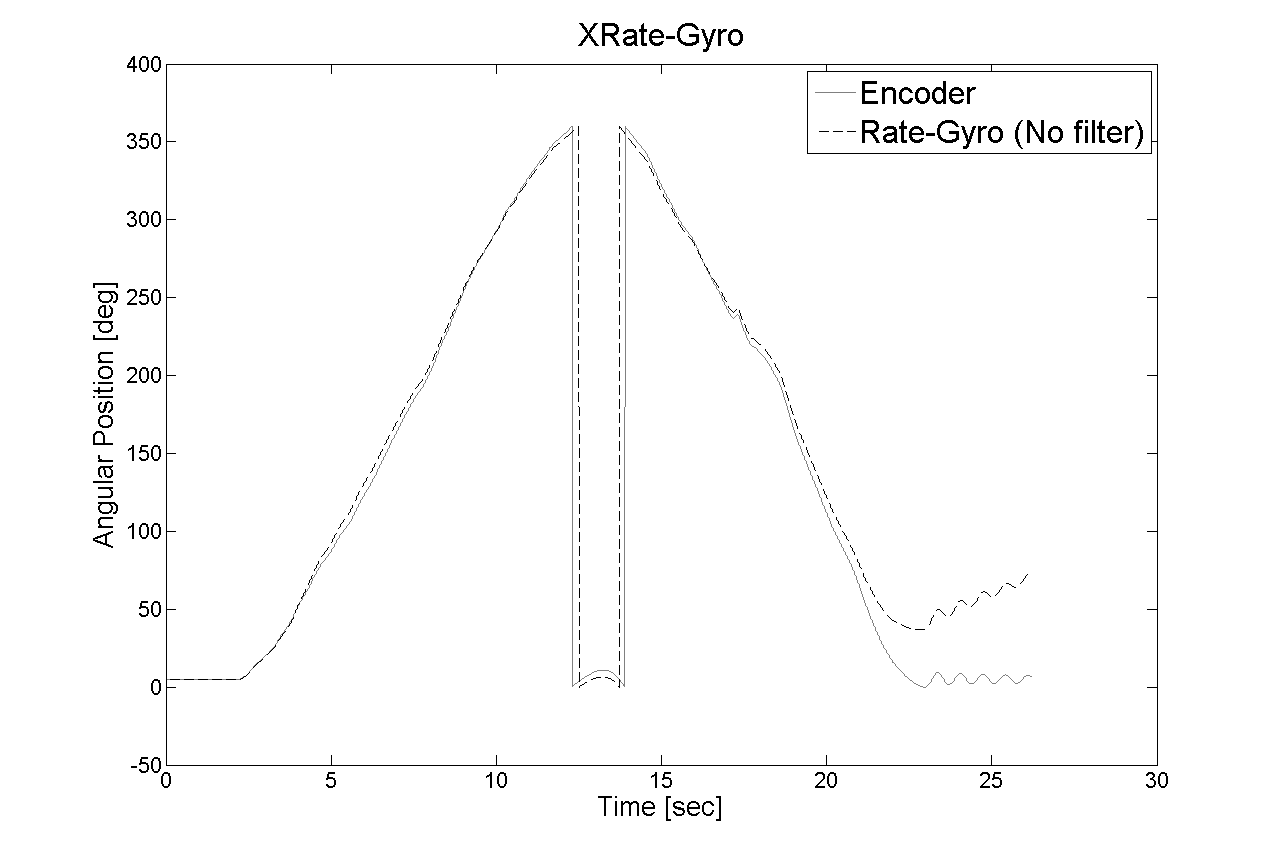
\includegraphics[width = 13cm]{Gyro_TimeDomain.png}
\caption{Angular Position vs. Time}
\label{Gyro_TimeDomain}
\end{center}
\end{figure}

\begin{figure}[hbt]
\begin{center}
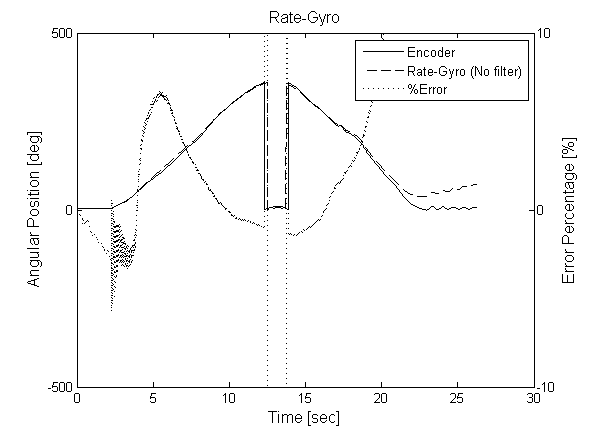
\includegraphics[width = 13cm]{Gyro_ErrorPercentage.png}
\caption{\% Error Percentage of Angular Position vs. Time}
\label{Gyro_ErrorPercentage}
\end{center}
\end{figure}

\begin{figure}[hbt]
\begin{center}
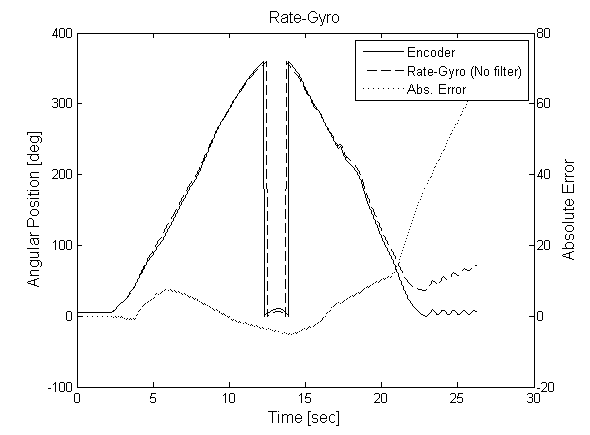
\includegraphics[width = 13cm]{Gyro_AbsError.png}
\caption{Absolute Error of Angular Position vs. Time}
\label{Gyro_AbsError}
\end{center}
\end{figure}


\subsubsection{Sensitivity}

As described above, there is no linear relationship between the voltage reported by the rate gyro and the angular position of the pendulum.  

\begin{figure}[hbt]
\begin{center}
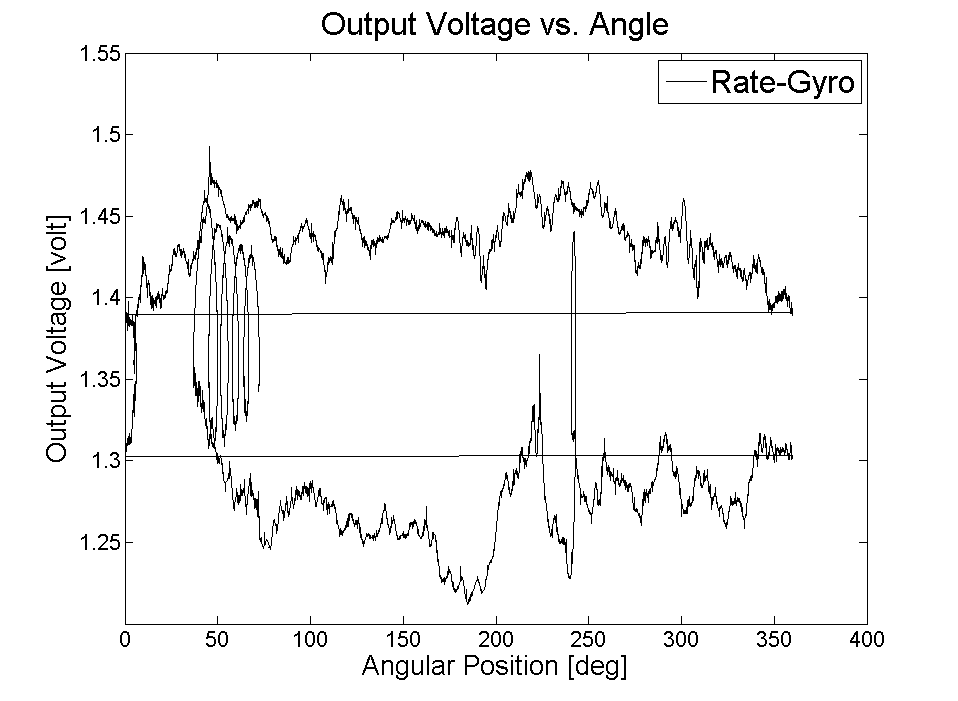
\includegraphics[width =12cm]{Gyro_Vol_vs_Angle.png}
\caption{Output Voltage vs. Angular Position}
\label{Gyro_Vol_vs_Angle}
\end{center}
\end{figure}

\subsubsection{Noise}

Because $\theta$ is given as a function of the sum of previous measurements, errors in $\theta$ are cumulative and will diverge from the true value over time.  This is reflected in time increasing variance, here expressed in terms of the number of measurements made.  Note that the following derivation neglects the variance in the zero rate which will only worsen performance and assumes that gyro variance is independent of time.

$$ \sigma_{\theta}(t) \approx \left( \frac{\sigma_{Gyro}^2}{\Sens_{Gyro}} \right) \left\{ \frac{t(1) - t(0)}{2} + \sum_{i = 1}^{n-1} \big( t(i) - t(i-1) \big) + \frac{t(n) - t(n-1)}{2} \right\} \approx \left( \frac{\sigma_{Gyro}^2}{\Sens_{Gyro}} \right) t$$

\emph{Where n is the sample taken at time, t.} \\

It is important to note, that despite this high variance, the actual output will look quite smooth because of the high degree of correlation between subsequent position estimates.  \\

The following trial was conducted for a fixed vertical pendulum angle, $\alpha = 0$.  Because our noise trial was done stationary, the gyro's lack of sensitivity to low frequency motion was not important, and its superior noise characteristics to the other sensors lead to very little noise in $\theta$.  In this trial, the Zero Rate was estimated from data within the first second.  Notice the slight discrepancy between the mean gyro voltage, and the zero rate.  This discrepancy leads to the divergent behavior seen in figure \ref{static_Gyro}.   Compared to the effect of zero rate drift, the effect of accumulating errors due to integration is essentially negligible.  

\begin{table}
\begin{center}
    \begin{tabular}{|c|c|}
        \hline
        ~                     & Actual \\ \hline
        $\sigma^2_{V_{Gyro}} \, (V^2)$              &  1.0179178 \e{-6}      \\ 
        $\sigma^2_{\theta} \, (rad^2)$             & 3.3233613 \e{-6}      \\ 
        $\mu_{V_{Gyro}} \, (V)$                &  1.360523703     \\ 
	$ ZeroRate_{Gyro} \, (V)$ 	     &  1.360478444 \\
        $\mu_{\theta} \, (rad)$               &  0.002894257     \\
	Peak to Peak $(V)$ &   0.013 \\
        Peak to Peak $(rad)$ & $1.665 \e{-4}$ \\
        \hline
    \end{tabular}
\caption{Observed Rate Gyro noise and resulting angle estimate for fixed $\theta = 0$.  Noise given for unfiltered data.}
\label{Noise_horizontal_T}
\end{center}
\end{table}

\begin{figure}
\begin{center}
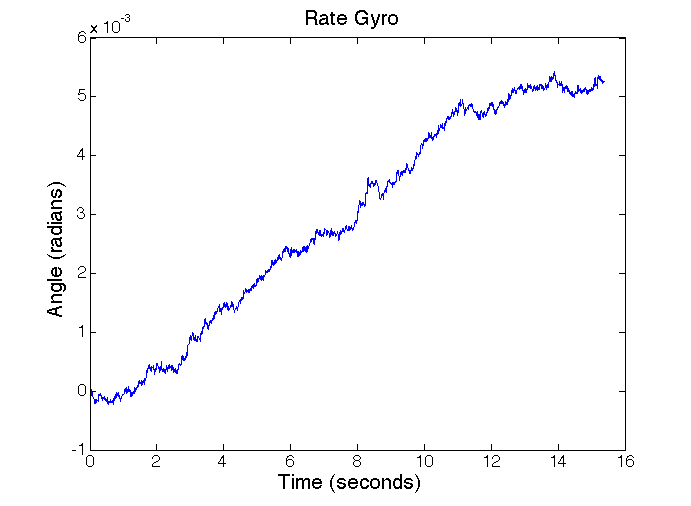
\includegraphics[width = 12cm]{rateGyro_Static.png}
\caption{Rate Gyro Angle estimate with static pendulum at $\theta = 0$}
\label{static_Gyro}
\end{center}
\end{figure}

\begin{figure}[hbt]
\begin{center}
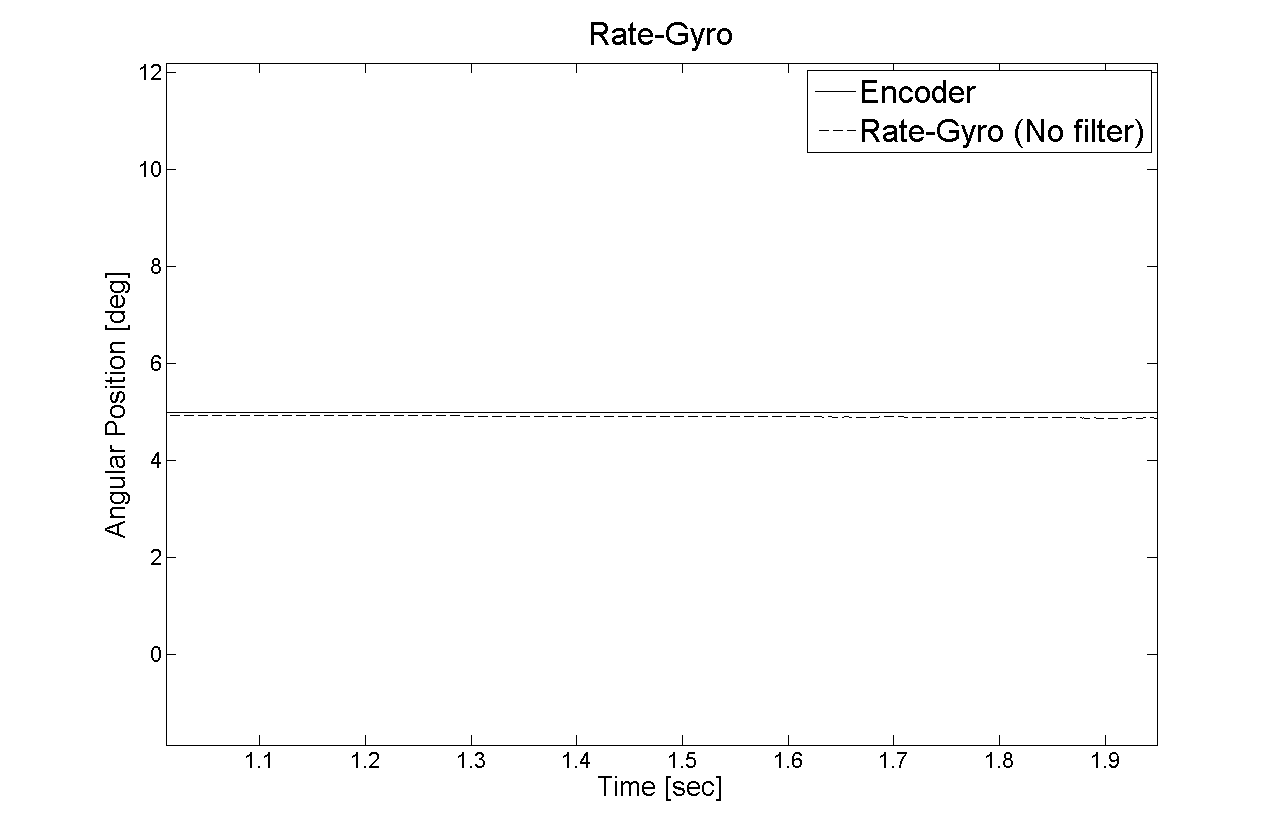
\includegraphics[width = 13cm]{Gyro_Peak2peak.png}
\caption{Angular Position vs. Time}
\label{Gyro_Peak2peak}
\end{center}
\end{figure}

\clearpage
%%%%%%%%%%%%%%%%%%%

\section{Filter Results}
We implemented four digital filters for our system to suppress the noise in our data:
\begin{enumerate}
\item Low Pass Filter
\item High Pass Filter
\item Moving Average Filter
\item Kalman Filter
\end{enumerate}
We looked at how the various filters performed and compared their performance along the following criteria:
\begin{itemize}
\item Steady State Output Variance

\item Response Time
\end{itemize}
As with any system there was a fine balance between low steady state noise and response time. Filters that could heavily suppress noise at steady state showed heavy lag when run. For the individual sensors we tried t arrive at a compromise where we could achieve sufficient noise suppression and took a hit on the lag aspect of the system. For complimentary filtering on the other hand, we tuned the system to have lower lag and settled for steady state noise. All these parameters were tuned subjectively, but for each filter and filter combination, a wide range of filter combinations were tried out and tested.\\

At at glance, the filtering results for high frequency noise can be seen in figure \ref{ss_noise_filtering}. The Bode plots were generated by comparing the input and output of the filters when feeding them a sinusoidal input. 100, logarithmically spaced, uniformly distributed frequencies between $10^{-2}$ Hz and $10^2$ Hz were used. The signals were fed into each filter and the corresponding amplitude ratios and phase differences were extracted. The results were then plotted.\\

 We tuned the filters to get minimal steady state variance, while not lagging the input signal by more than 0.03 seconds. The phase lag was arbitrarily decided upon. Each subsection further looks into how each filter was implemented, while the appendix has the matlab code of the implementation\footnote{See Appendix: lab6Filters.m for individual filter implementation}. While working with data offline, it is important to ensure that the filtering processes are causal- i.e. they do not access information that would normally be unavailable to them.\\

Each filter was designed to use a different algorithm, the most interesting being the Kalman filter which uses posterior prediction to account for system and sensor noise. This was an interesting implementation for us as the filter is very different from any other filter we have used in the various lab experiments conducted. It is explained in detail under the Kalman Filter subsection.\\


\begin{figure}[hbt]
\begin{center}
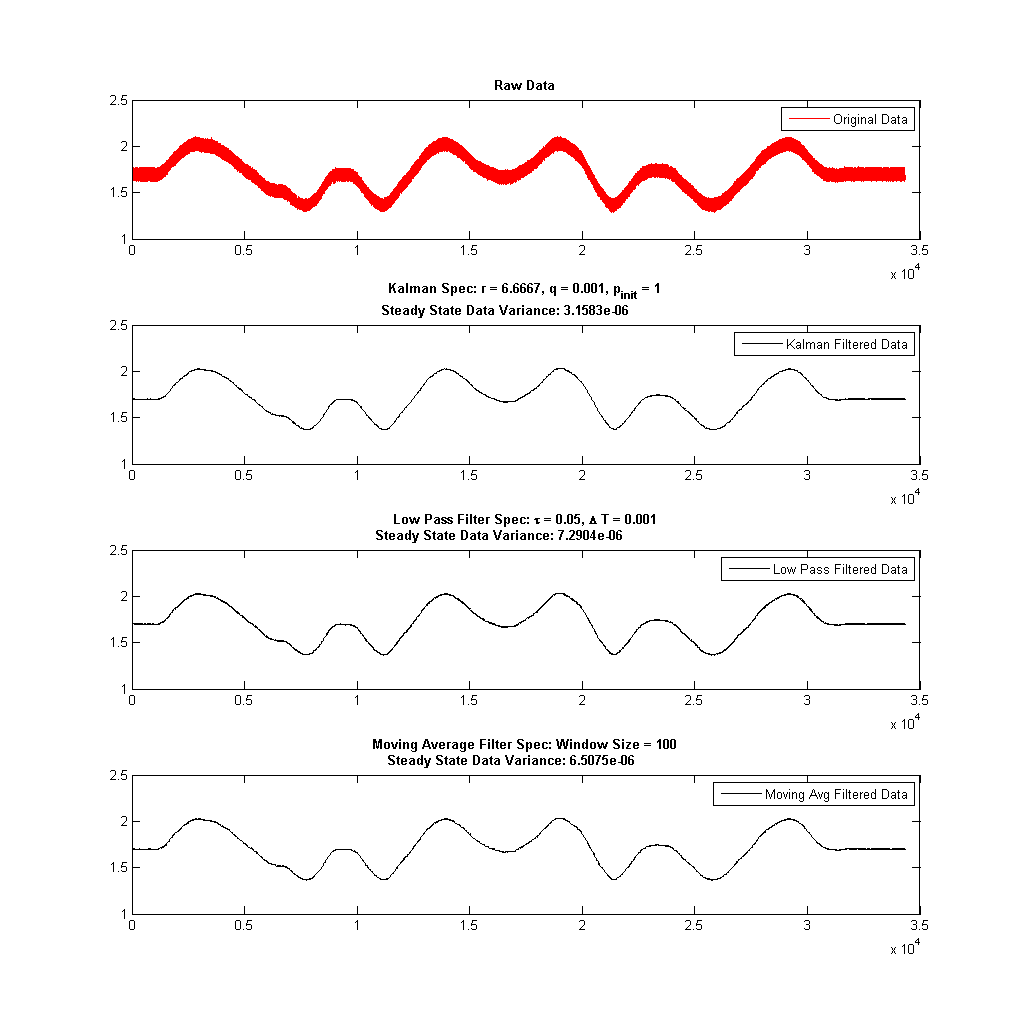
\includegraphics[width = 16cm]{ss_noise_filtering.png}
\caption{High frequency noise suppression by the three filters - while tuning each filter, we we looked to minimize the steady state noise while trying to keep the peaks of the filtered data as close to the real peaks as possible. The Data has a steady-state variance of 0.02 V, after filtering, the variance is reduced by almost $10^4$  in every case.}
\label{ss_noise_filtering}
\end{center}
\end{figure}

\clearpage

\subsection{Low Pass Filter}
The low pass filter rejects the high frequency component of a signal. It acts as a high inertia-damper to the signal. It has a transfer function given by: 
$$H(s) = \frac{1}{s\tau + 1}$$
Where $\tau$ represents the corner frequency. Digitally, it can be implemented through the following algorithm:
\begin{verbatim}
double lowPass(double x[], double dt, double tau){
   double output[x.length];
   double alpha = dt / (tau + dt);
   output[0] = x[0];
   for (int i= 1; i < x.length; i++)
       output[i] = alpha * x[i] + (1-alpha) * output[i-1];
   return output
}
\end{verbatim}

The Bode plot of the digital low pass filter can be seen in figure \ref{bode_LPF}. As you can see, its response is similar to a physical low pass filter. 


\begin{figure}[hbt]
\begin{center}
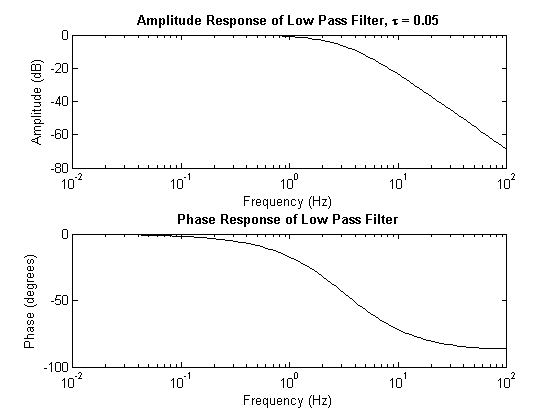
\includegraphics[width = 10cm]{bode_LPF}
\caption{Bode plot of the Low Pass Filter}
\label{bode_LPF}
\end{center}
\end{figure}

\clearpage



\subsection{Moving Average Filter}
As the name suggests, the moving average filter, holds on to the average of a range values. The length of the range is called the filter's Window ($\mu_{size}$). The larger the window, the more number of points that are averaged. High signal variance reduction requires a larger window, which in turn means that more points would have to be sampled to produce an output. This introduces lag into the system. Algorithmically, the filter is implemented as follows:

\begin{verbatim}
double movAvg(double x[], int windowSize){
   double output[x.length];   
   for (int i= 0; i < x.length; i++){
        if(i <= MAvgWindowSize)
            output[i] = sum(x[0] to x[i])/(i+1);
        else
            output[i] = sum(x[i-MAvgWindowSize] to x[i])/(MAvgWindowSize+1);
   }
   return output
}
\end{verbatim}

Looking at the Bode plot of the filter, (figure \ref{bode_MAvgF}), we see a very uniform magnitude and phasic response followed by a sharp drop at higher frequencies for the magnitude plot and an unusual spike for the phase plot. This drop and spike are the result of the filter window being so large,it encompasses the entire sinusoidal input itself - resulting in something similar to aliasing.

\begin{figure}[hbt]
\begin{center}
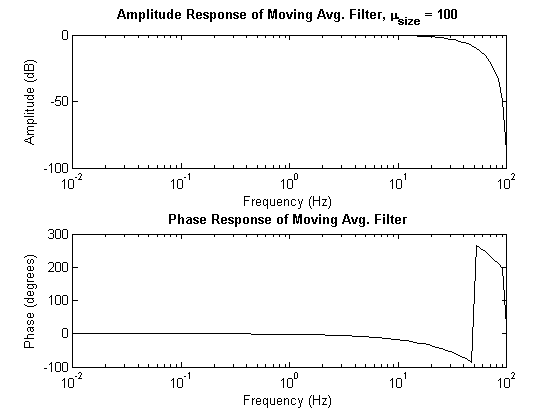
\includegraphics[width = 10cm]{bode_MAvgF}
\caption{Bode plot of the Moving Average Filter}
\label{bode_MAvgF}
\end{center}
\end{figure}
 
\clearpage

\subsection{Kalman Filter}
A Kalman filter is used to make predictions in a noisy environment. At its core, it tries estimate the current step given a prediction and an observation. It uses the concept of covariance based weighting to decide how much it can rely on the observations - which are noisy, and how much it can rely on its prediction, given uncertain model of the system. The ordinary Kalman filter, used here is a linear estimator - for non-linear filtering an extended Kalman filter can be used, but that is beyond the scope of the lab assignment.\\

The Kalman filter consists of the following steps:
\begin{itemize}
\item Initialization - This is the preprocessing step of the Kalman filter. We set our estimates of the process noise ($q$), sensor noise ($r$) and the initial state ($X_0$). We also require an update model - some way to decide how the state will change based of given conditions. For a senor-system, we do not require a state propagation model, we assume that it changes its state solely due to external, uncontrolled factors.
$$X_t - \text{State at time }t$$
$$X_0 = observations_{t = 0}$$
$$q - \text{Process Noise}$$
$$r - \text{Sensor Noise}$$
$$p - \text{Estimated Noise}$$
$$X_{t-1} \rightarrow X_t - \text{State propagation model}$$

\item Prediction - Based on the state propagation model, we can now predict what the system will look like in the future. In the case of the sensor model, since we have no state propagation model, this means that effectively we expect the state to remain constant.
$$\hat{X_{t}} -\text{Predicted state at time }t$$
$$\hat{X_{t}} = X_{t-1}$$

\item Observation - We now look at our noisy sensors to sense what the state looks like at the moment. This observation is treated with skepticism as we know that noise pollutes our observations. We additionally have to adjust our estimated error.
$$observations_{t}$$
$$p = p+q$$

\item Sate Estimation - Based on our prediction, we can propagate our state model. We would like to move the state by some belief value towards the difference of our observations and prediction. This belief value is called the \emph{Kalman Gain} ($\kappa$) and it is the ratio of the previous state's error estimate to the total uncertainty of the current prediction and observation. We have to update this gain every time. As noise propagates into the system, our certainty of the signal update will continue to degrade steadily. 
$$\kappa =  \frac{p}{p+r}$$
$$X_{t} = X_{t-1} + \kappa * (observations_t- \hat{X}_t)$$
We now need to also update the error estimate of the current state, this is simply given as:
$$p = (1 - \kappa) * p$$
\end{itemize}

The digital implementation of the of the Kalman filter is as follows:
\begin{verbatim}
class State{
    double x;
    double error;
}
State Simple_Kalman(measurement, State x_old, r, q){
    double p_new = x_old.error + q;
    K = p_new/(p_new+r);
    State x_new;
    x_new.x = x_old.x + K*(measurement - x_old.x);
    x_new.error = (1-K)*p_new;
}
\end{verbatim}

The Bode plot of the filter can be seen in figure \ref{bode_KF}. The plot shows a drop very similar to a first order filter once we hit its corner frequency. What is interesting to note is that its phase-lag increase is more gradual than the low pass filter. 


\begin{figure}[hbt]
\begin{center}
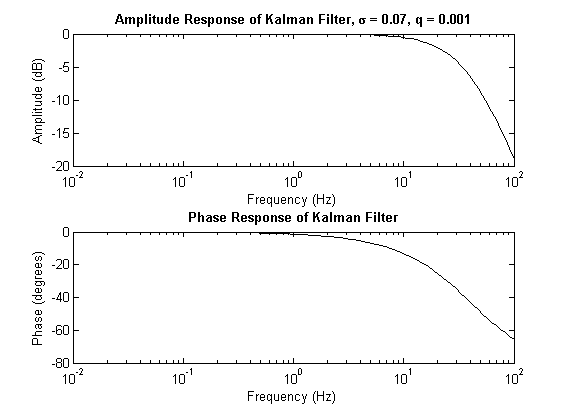
\includegraphics[width = 12cm]{bode_KF}
\caption{Bode plot of the Kalman Filter}
\label{bode_KF}
\end{center}
\end{figure}

\subsection*{Determining System Fidelity}
In order to determine how much we could trust the signal, we had to find some measure of the output fidelity, $r$. This was done by looking at the steady state variance, $\sigma$, of the signal when the accelerometer experiences no accelerative forces. With the variance computed, we get an idea of how noisy the sensor is.\\

We also found that including some, minuscule, process noise was also very helpful in getting good results. No process noise implies that State Transitions are perfect - in our case it is clearly not the case. Thus we set $q$ to be some arbitrarily small value (order $10^2$ times less than the sensor noise, $r$).

\subsection*{More Complicated Kalman Filters and Sensor Fusion}
Kalman filters essentially work in the state-space domain, it is easy to convert this 1-D signal filter to a multi-input, multi-output filter. The system noise changes from a single variance estimate to covariance matrices. Additionally non-independent noise, i.e., noise which leaks from one sensor onto another can be modeled. However, we specifically assumed the noise distribution in our system to be independent, that way, it the more advanced Kalman filter will behave just the same way as a set of $N$1-D Kalman Filters.\\

Another use of the Kalman filter is to combine accelerometer and gyroscopic data to get a tilt estimate. This is an interesting idea as we can dynamically set each inputs Kalman gain and accordingly combine data in a more controllable way than the traditional additive sensor fusion. However we did not have enough time to explore this path and it remains, at this point, for future work.


\subsection{High Pass Filter}
Algorithm:
\begin{verbatim}
double highPass(double x[], double dt, double tau){
   double output[x.length];
   double alpha = tau / (tau + dt);
   output[0] = x[0];
   for (int i= 1; i < ; i++)
       output[i] = alpha * (output[i-1] + x[i] - x[i-1]);
   return output
}
\end{verbatim}

\begin{figure}[hbt]
\begin{center}
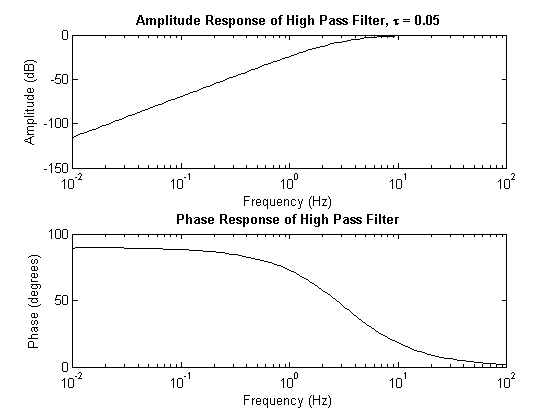
\includegraphics[width = 10cm]{bode_HPF}
\caption{Bode plot of the High Pass Filter}
\label{bode_HPF}
\end{center}
\end{figure}

\clearpage

\subsection{Sensor Fusion:- Filter Perspective}

\begin{figure}[hbt]
\begin{center}
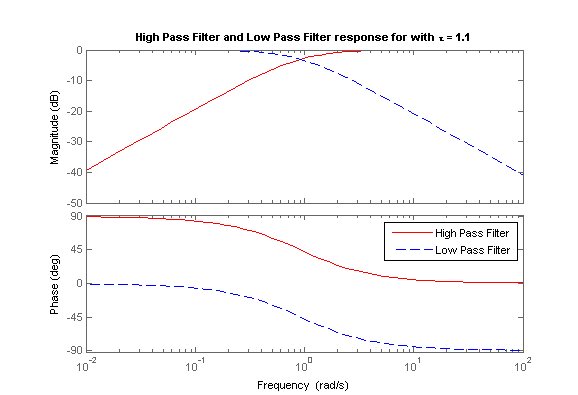
\includegraphics[width = 12cm]{bode_SensorFusion}
\caption{Bode plot of the Sensor Fusion scheme}
\label{bode_SF}
\end{center}
\end{figure}

\clearpage
%%%%%%%%%%%%%%%%%%%


\section{Higher Frequency Characterization}

To determine the range of motiion that could be measured, the pendulum was moved through a full rotation at highspeed. To determine the magnitude, phase, and other performance measures as a function of frequency, the pendulum was allowed to oscillate naturally with the shaft collars at differect positions along its length to alter the center-of-mass. Then, the pendulm was manually oscillated at several frequencies (as consistently as possible). In all cases the low-pass filter time constant and the kalman filter variance were kept constant (0.05 and 0.07, respectively) for all of the accelerometer calculations. The time constant of the high-pass filter used with the rate gyro's was changed with every trial.\\  

The three filtering methods used with the accelerometers had similar performance overall, but the kalman filter tended to have lower phase lag, as shown in figure \ref{kalman_lag}. Therefore, all performance measures given in the following sections are based on the kalman filter.\\

\begin{figure}[hbt]
\begin{center}
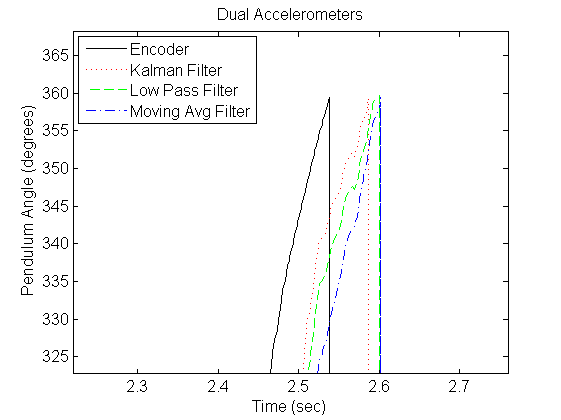
\includegraphics[width = 12cm]{Example_Kalman_Lag.png}
\caption{Comparison of filtering methods during high-speed, full rotation of pendulum}
\label{kalman_lag}
\end{center}
\end{figure}

\subsection{Horizontal Accelerometer}

\subsubsection{High Frequency}

Figure \ref{full_horizontal} shows the angular range of the horizontal accelerometer when the pendulum undergoes a full rotation at high speed. The acclerometer was capable of an ouput range of $\pm$90$^{\circ}$ and is capable of distinguishing direction of rotation, but in this case the encoder was outputting 0$^{\circ}$ to 360$^{\circ}$, leading to some disagreement. Had the encoder been outputting -180$^{\circ}$ to 180$^{\circ}$, there would be more agreement within the accelerometer's range.\\

Figure \ref{normal_horizontal} shows one test of the pendulum oscillating naturally. The horizontal accelerometer's magnitude was under 10\% for all tests up to 1.7606 Hz, but the phase lag was never below 10$^{\circ}$. The smallest lag was 23.6469$^{\circ}$ at 1.3902 Hz. Also, the average steady-state error was 6.955$^{\circ}$, which may have been caused by the pendulum not being perfectly vertical when the tests began.\\ 

\begin{figure}[hbt]
\begin{center}
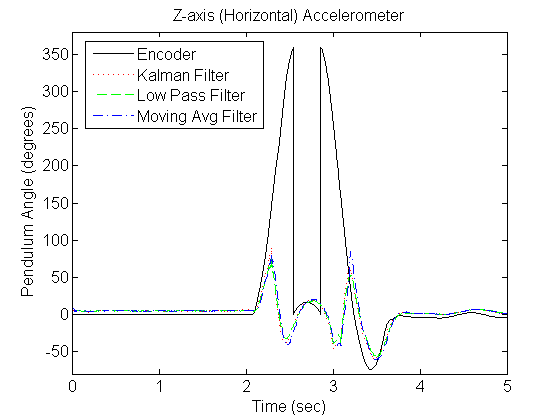
\includegraphics[width = 12cm]{FullRotation_Horizontal.png}
\caption{Horizontal accelerometer with high-speed, full rotation of pendulum}
\label{full_horizontal}
\end{center}
\end{figure}

\begin{figure}[hbt]
\begin{center}
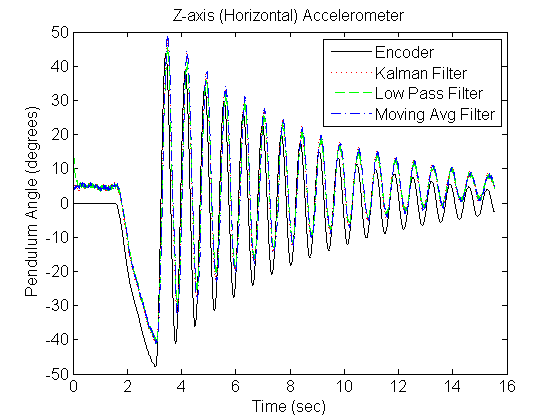
\includegraphics[width = 12cm]{NormalMass_Horizontal.png}
\caption{Horizontal accelerometer at pendulum's natural frequency}
\label{normal_horizontal}
\end{center}
\end{figure}

Figure \ref{horizontalBode} shows the experimentally derived bode plot for the horizontal accelerometer and tables \ref{horizontal_tableA} and \ref{horizontal_tableB} give the performance measures. The magnitude of the angular output is close to unity until around 1.5 Hz, and then drops significantly. The voltage output of the accelerometer (and therefore the angle calculated) is not only dependant on the $\theta$, but also $\ddot{\theta}$ (eqn. \ref{Vout}).  $\ddot{\theta}$ is a function of frequency (eqn. \ref{thetadoubledot}), so we expect that as the frequency increases, the accuracy of the sensor will diminish. The filters produce some minimum level of time lag, so as the frequency increases, the phase difference that the time lag corresponds to increases. \\

\begin{equation}
V_{out} = V_{bis} + S(-a_0 cos(\theta) + r\ddot{\theta} - g sin(\theta))
\label{Vout}
\end{equation}

\begin{equation}
\ddot{\theta} = -4 \pi^2 f^2 \theta_0 cos(2\pi f t)
\label{thetadoubledot}
\end{equation}

\begin{figure}[hbt]
\begin{center}
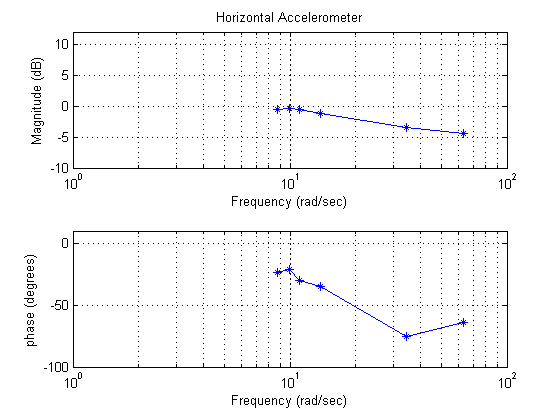
\includegraphics[width = 14cm]{HorizontalBode.png}
\caption{Horizontal accelerometer's frequency response}
\label{horizontalBode}
\end{center}
\end{figure}

\begin{table}
\begin{center}
    \begin{tabular}{|c|c|c|c|}
        \hline
        Frequency (Hz)  & Magnitude (dB) & Phase (deg.) & \% Magnitude Error \\ \hline
	1.3902  & -0.4914  & -23.6469 & 5.5\\
       1.5846  & -0.3881  & -32.6575 & 4.37 \\
	1.7606  & -0.5181  & -29.7897  & 5.79  \\
	2.2029 &  -1.1301 & -34.6961 &  12.2  \\
	5.4772 & -3.4578  & -75.4212 & 32.6519  \\
	10.0358 & -4.4619 & -64.1289 & 39.6921 \\
        \hline
    \end{tabular}
\caption{Horizontal accelerometer performance measures - A}  
\label{horizontal_tableA}
\end{center}
\end{table}

\begin{table}
\begin{center}
    \begin{tabular}{|c|c|c|c|}
        \hline
        Frequency (Hz)  & Voltage Noise (V) & Observed Angle Noise (deg.) & Steady-State Error (deg.) \\ \hline
	1.3902  & 0.138  & 2.18 & 5.076\\
       1.5846  & 0.142  & 1.471 & 3.128 \\
	1.7606  & 0.136 & 1.609 & 6.1605  \\
	2.2029 & 0.134  & 1.99 & 7.7865   \\
	5.4772 & 0.343  & 2.223 & 6.842  \\
	10.0358 & 0.677 & 1.524 & 12.739 \\
        \hline
    \end{tabular}
\caption{Horizontal accelerometer performance measures - B}  
\label{horizontal_tableB}
\end{center}
\end{table}


\subsubsection{High Frequency with Horizontal Arm Disturbance}

\clearpage
%%%%%%%%%%%%%%%%%%%%%

\subsection{Vertical Accelerometer}
\subsubsection{High Frequency}

Figure \ref{full_vertical} shows the angular range of the vertical accelerometer when the pendulum undergoes a full rotation at high speed. The accelerometer was capable of an ouput range of 0$^{\circ}$to 152.4$^{\circ}$. However, it is not capable of distinguishing direction of rotation (ie. it can't distinguish positive from negative angles from the intial vertical position). \\

Figure \ref{normal_horizontal} shows one test of the pendulum oscillating naturally. In this case, the magnitude of angle output matched the encoder decently, but because it can't distinguish negative angles, it isn't accurate for anything but magnitude. The magnitude was under 10\% for all tests up to 1.7606 Hz (though it tended to be slightly greater than for the horizontal accelerometer), but the phase lag was never below 10$^{\circ}$ (at 5.4772 Hz the phase lag is only 9.8590$^{\circ}$, but this is likely a misleading result caused by the noise from manually shaking the pendulum). The smallest lag was 20.7696$^{\circ}$ at 1.3902 Hz. Also, the average steady-state error was 9.479$^{\circ}$. This is greater than with the horizontal accelerometer and is likely caused by the pendulum not being perfectly vertical at the start of the test, and greater observed noise in the anglular output.\\ 

\begin{figure}[hbt]
\begin{center}
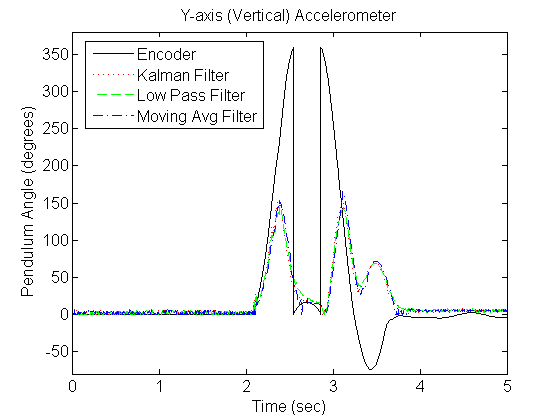
\includegraphics[width = 12cm]{FullRotation_Vertical.png}
\caption{Vertical accelerometer with high-speed, full rotation of pendulum}
\label{full_vertical}
\end{center}
\end{figure}

\begin{figure}[hbt]
\begin{center}
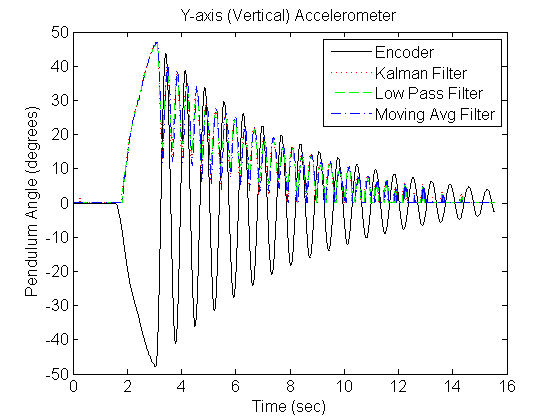
\includegraphics[width = 12cm]{NormalMass_Vertical.png}
\caption{Vertical accelerometer at pendulum's natural frequency}
\label{normal_vertical}
\end{center}
\end{figure}

Figure \ref{verticalBode} shows the experimentally derived bode plot for the vertical accelerometer and tables \ref{vertical_tableA} and \ref{vertical_tableB} give the performance measures. The magnitude of the angular output is close to unity until about 1.5 Hz, then it drops slightly before increasing. As mentioned with the horizontal accelerometer, voltage output  (and therefore the angle calculated) is not only dependant on the $\theta$, but also $\ddot{\theta}$ (eqn. \ref{Vout}).  $\ddot{\theta}$ is a function of frequency (eqn. \ref{thetadoubledot}), so we expect that as the frequency increases, the accuracy of the sensor will diminish. The increasing magnitude at higher frequencies may be attributed to the greater level of noise with this sensor, and the issues related to its inability to show direction of motion. The filters produce some minimum level of time lag, so as the frequency increases, the phase difference that the time lag corresponds to increases. \\


\begin{figure}[hbt]
\begin{center}
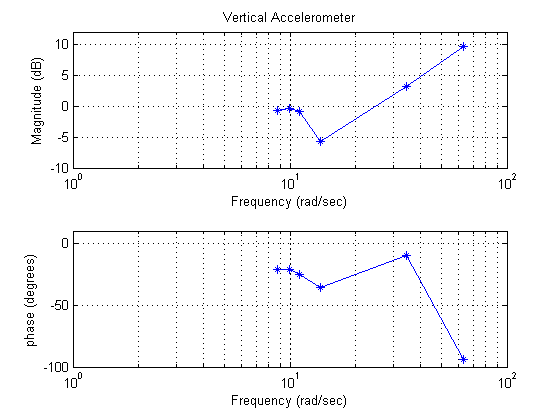
\includegraphics[width = 14cm]{VerticalBode.png}
\caption{Vertical accelerometer's frequency response}
\label{verticalBode}
\end{center}
\end{figure}


\begin{table}
\begin{center}
    \begin{tabular}{|c|c|c|c|}
        \hline
        Frequency (Hz)  & Magnitude (dB) & Phase (deg.) & \% Magnitude Error \\ \hline
	1.3902  & -0.7497  & -20.7696 & 8.27\\
       1.5846  & -0.3428  & -21.3914 & 3.87 \\
	1.7606  & -0.9113 & -25.1945 & 9.96  \\
	2.2029 & -5.6566  & -36.0839 & 47.86   \\
	5.4772 & 3.2533  & -9.8590 & 45.6211  \\
	10.0358 & 9.7344 & -93.9352 & 213.6681 \\
        \hline
    \end{tabular}
\caption{Vertical accelerometer performance measures - A}  
\label{vertical_tableA}
\end{center}
\end{table}

\begin{table}
\begin{center}
    \begin{tabular}{|c|c|c|c|}
        \hline
        Frequency (Hz)  & Voltage Noise (V) & Observed Angle Noise (deg.) & Steady-State Error (deg.) \\ \hline
	1.3902  & 0.029  & 4.426 & 4.7005\\
       1.5846  & 0.069  & 3.0877 & 2.74 \\
	1.7606  & 0.038 & 1.759 & 8.9485  \\
	2.2029 & 0.118  & 1.05 & 9.035   \\
	5.4772 & 0.744  & 1.47 & 12.195  \\
	10.0358 & 0.537 & 13.48 & 19.255 \\
        \hline
    \end{tabular}
\caption{Vertical accelerometer performance measures - B}  
\label{vertical_tableB}
\end{center}
\end{table}


\subsubsection{High Frequency with Horizontal Arm Disturbance}
\clearpage
%%%%%%%%%%%%%%%%%%%%%
\subsection{Two Accelerometers}
\subsubsection{High Frequency}

Figure \ref{full_Dual} shows the angular range using the atan2 function with two accelerometers. The accelerometer was capable of an ouput range from 0$^{\circ}$to 359.6$^{\circ}$, following the encoder through the full rotation. However, while this method can cover a full circle, the user has too choose whether they want it output as 0$^{\circ}$ to 360$^{\circ}$ or -180$^{\circ}$ to 180$^{\circ}$. In this case we chose 0$^{\circ}$ to 360$^{\circ}$, which results in step changes when the pendulum is oscillating near 0. For the natural and forced oscillation tests, we chose instead to use -180$^{\circ}$ to 180$^{\circ}$ to cover the full range of the pendulum's motion. \\

Figure \ref{normal_dual} shows one test of the pendulum oscillating naturally. The dual encoder method matches the magnitude well in both directions, but there is still some steady-state error . Like the previous accelerometers, the magnitude was under 10\% for all tests up to 1.7606 Hz, but the phase lag was never below 10$^{\circ}$. Because it depends on the output of the two accelerometers, it makes sense that the magnitude and phase are similar, but this method gives better range. The smallest lag was 22.89$^{\circ}$ at 1.3902 Hz. The average steady-state error was 6.6766$^{\circ}$, which is less than the two individual accelerometers.\\ 

\begin{figure}[hbt]
\begin{center}
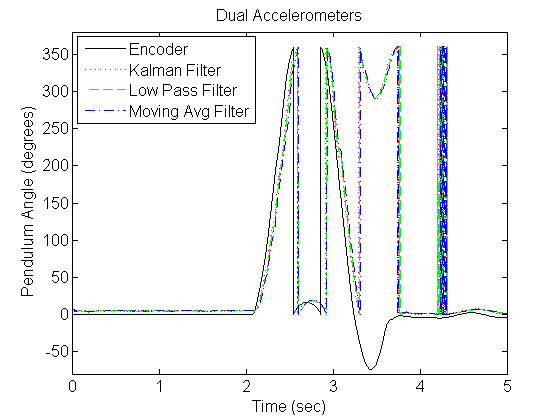
\includegraphics[width = 12cm]{FullRotation_Dual.png}
\caption{Dual accelerometers with high-speed, full rotation of pendulum}
\label{full_Dual}
\end{center}
\end{figure}

\begin{figure}[hbt]
\begin{center}
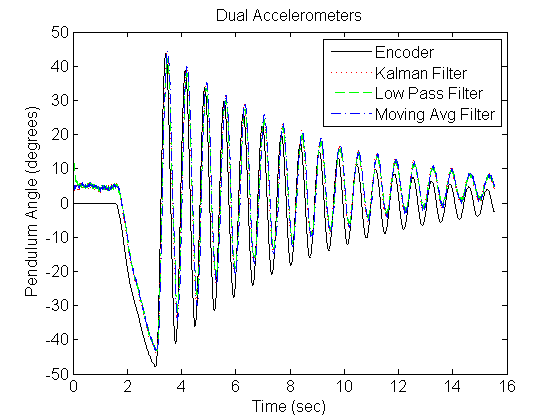
\includegraphics[width = 12cm]{NormalMass_Dual.png}
\caption{Dual accelerometers at pendulum's natural frequency}
\label{normal_dual}
\end{center}
\end{figure}

Figure \ref{dualBode} shows the experimentally derived bode plot for the atan2 function with two accelerometers and tables \ref{dual_tableA} and \ref{dual_tableB} give the performance measures. The bode plot generally resembles that of the horizontal acceleromter with the magnitude of the angular output is close to unity until about 1.5 Hz before dropping at a constant slope. Because this method is dependant on both accelerometers, it is subject to their sensitivity to $\ddot{\theta}$ and has a time lag caused by the filters that exacerbates the phase lag as frequency increases. \\

\begin{figure}[hbt]
\begin{center}
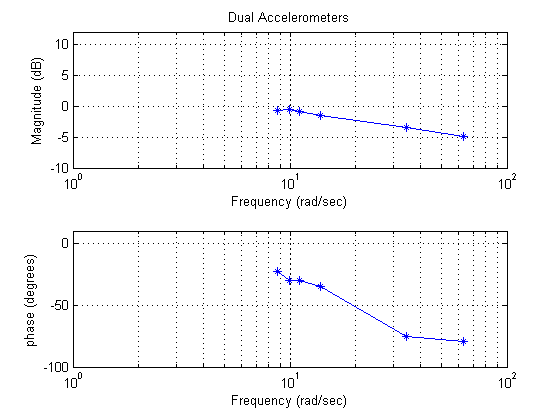
\includegraphics[width = 14cm]{DualBode.png}
\caption{Dual accelerometers' frequency response}
\label{dualBode}
\end{center}
\end{figure}


\begin{table}
\begin{center}
    \begin{tabular}{|c|c|c|c|}
        \hline
        Frequency (Hz)  & Magnitude (dB) & Phase (deg.) & \% Magnitude Error \\ \hline
	1.3902  & -0.7455  & -22.89 & 8.22\\
       1.5846  & -0.6154  & -30.0906 & 6.84\\
	1.7606  & -0.8154 & -29.7897 & 8.96  \\
	2.2029 & -1.5767  & -34.6961 & 16.6   \\
	5.4772 & -3.5125  & -74.9282 & 33.0799  \\
	10.0358 & -4.8405 & -79.4837 & 42.2778 \\
        \hline
    \end{tabular}
\caption{Dual accelerometer performance measures - A}  
\label{dual_tableA}
\end{center}
\end{table}

\begin{table}
\begin{center}
    \begin{tabular}{|c|c|c|c|}
        \hline
        Frequency (Hz)  & Voltage Noise (V) & Observed Angle Noise (deg.) & Steady-State Error (deg.) \\ \hline
	1.3902  & 0.167  & 1.26 & 4.9211\\
       1.5846  & 0.211  & 1.397 & 2.5075 \\
	1.7606  & 0.174 & 1.529 & 6.1495  \\
	2.2029 & 0.252  & 1.22 & 6.1335   \\
	5.4772 & 1.087  & 1.398 & 6.8185  \\
	10.0358 & 1.214 & 1.572 & 13.5295 \\
        \hline
    \end{tabular}
\caption{Dual accelerometer performance measures - B}  
\label{dual_tableB}
\end{center}
\end{table}

\subsubsection{High Frequency with Horizontal Arm Disturbance}

\clearpage
%%%%%%%%%%%%%%%%%%%%%
\subsection{Rate Gyro}
\subsubsection{High Frequency}

To calculate the angular position with the rate gyros, the voltage output was converted to angular rate as mentioned previously, and then integrated using a Riemann sum method. \\

Figures \ref{full_gyro} and \ref{full_gyro45} show the angular range using the standard rate gyro and the 4.5 gyro, respectively. The standard gyro output to 130.4$^{\circ}$ while the 4.5 gyro only reached 96.08$^{\circ}$. In both cases the gyro's output voltage saturated, effectively limiting the max rate that they could output (as shown by the differences in slope between the encoder and gyro). This saturation is a large cause of the steady-state error at the end of the test.\\

Figures \ref{normal_gyro} and \ref{normal_gyro45} show tests of the pendulum oscillating naturally. The 4.5 gyro experienced saturation in every oscillation test, leading to very large steady-state errors. However, both gyros tended to show very minimal magnitude errors. The standard gyro was well under 10\% for all frequencies tested, and the 4.5 gyro was only over 10\% at 2.2029 and 5.4772 Hz, but back under 10\% at 10.0358 Hz. The phase difference of both gyros was always under 10$^{\circ}$, in fact never going above 2.71$^{\circ}$. The voltage noise for both was also very small, chiefly because of the low-pass filter integrated into the gyro chip. Additionally, the integration method resulted in effectively no noise in the angle output. Even when there was a spike in the voltage that caused a spike in the angular rate, it was integrated over such a short time period that the effect on the angular position output was minimal. Figures \ref{horizontalNoise} and \ref{gyroNoise} show a comparison of the voltage noise from the horizontal accelerometer and the much smaller noise from the rate gyro. Figure \ref{gyroAngleNoise} shows that even at the point when the voltage noise was greatest, the angular output showed no noise compared to the encoder. However,  steady-state error of the standard gyro was not much different from the accelerometers and was much worse for the 4.5 gyro, largely because of the saturation issues mentioned previously.\\ 

\begin{figure}[hbt]
\begin{center}
\includegraphics[width = 12cm]{FullRotation_Gyro.png}
\caption{Rate gyro with high-speed, full rotation of pendulum}
\label{full_gyro}
\end{center}
\end{figure}

\begin{figure}[hbt]
\begin{center}
\includegraphics[width = 12cm]{FullRotation_Gyro45.png}
\caption{4.5 Rate gyro with high-speed, full rotation of pendulum}
\label{full_gyro45}
\end{center}
\end{figure}

\begin{figure}[hbt]
\begin{center}
\includegraphics[width = 12cm]{NormalMass_Gyro.png}
\caption{Rate gyro at pendulum's natural frequency}
\label{normal_gyro}
\end{center}
\end{figure}

\begin{figure}[hbt]
\begin{center}
\includegraphics[width = 12cm]{NormalMass_Gyro45.png}
\caption{4.5 Rate gyro at pendulum's natural frequency}
\label{normal_gyro45}
\end{center}
\end{figure}

\begin{figure}[hbt]
\begin{center}
\includegraphics[width = 12cm]{Example_Horizontal_Noise.png}
\caption{Typical voltage noise of the horizontal acceleromter}
\label{horizontalNoise}
\end{center}
\end{figure}

\begin{figure}[hbt]
\begin{center}
\includegraphics[width = 12cm]{Example_Gyro_Noise.png}
\caption{Voltage noise of the rate gyro}
\label{gyroNoise}
\end{center}
\end{figure}

\begin{figure}[hbt]
\begin{center}
\includegraphics[width = 13cm]{Example_Gyro_AngleNoise.png}
\caption{At the point of maximum voltage noise from the rate gyro, angular output shows no noise compared to the encoder}
\label{gyroAngleNoise}
\end{center}
\end{figure}

Figures \ref{gyroBode} and \ref{gyro45Bode} show the experimentally derived bode plot for the standard and 4.5 gryos, and tables \ref{gyro_tableA} through \ref{gyro45_tableB} give the performance measures. The bode plot for both stays very flat across the frequency range tested, with only a small drop in the magnitude of the 4.5 gyro. The phase for both was very small, and in some cases was even  about zero or leading. This is likely a somewhat misleading effect of using right-Riemann sums for integration, causing the response plot to shift to the left and upwards slightly. The small effect of these high frequencies is to be expected. The output of the gyro is based on the coriolis acceleration of the proof-mass which shows up in the pick-up direction of the proof-mass. The excitation frequency in the primary direction is known (and is the same as the coriolis) and can be used to filter out unwanted excitations at other frequencies, and then a demodulator is used to extract only the amplitude in the pick-up direction with (ideally) no dependancy on the outside excitation frequency. \\ 

\begin{figure}[hbt]
\begin{center}
\includegraphics[width = 14cm]{GyroBode.png}
\caption{Rate gyro's frequency response}
\label{gyroBode}
\end{center}
\end{figure}

\begin{figure}[hbt]
\begin{center}
\includegraphics[width = 14cm]{Gyro45Bode.png}
\caption{4.5 gyro's frequency response}
\label{gyro45Bode}
\end{center}
\end{figure}

\begin{table}
\begin{center}
    \begin{tabular}{|c|c|c|c|c|}
        \hline
        Frequency (Hz) & tau & Magnitude (dB) & Phase (deg.) & \% Magnitude Error \\ \hline
	1.3902 & 2200 & -0.1300  & 0 & 1.4859\\
       1.5846 & 7500 & -0.1441  & 2.72E-13 & 1.6347\\
	1.7606 & 10000 & -0.0811 & 0.1665 & 0.9185  \\
	2.2029& 12000 & -0.1460  & -0.6067 & 1.6654   \\
	5.4772&20000 & -0.0749  & -0.6320 & 0.8537  \\
	10.0358& 165 & -0.0440 & 2.7097 & 0.4544 \\
        \hline
    \end{tabular}
\caption{Rate gyro performance measures - A}  
\label{gyro_tableA}
\end{center}
\end{table}

\begin{table}
\begin{center}
    \begin{tabular}{|c|c|c|c|}
        \hline
        Frequency (Hz)  & Voltage Noise (V) & Observed Angle Noise (deg.) & Steady-State Error (deg.) \\ \hline
	1.3902  & 0.009  & 0 & 1.562\\
       1.5846  & 0.007  & 0 & 6.065 \\
	1.7606  & 0.009 & 0 & 11.843  \\
	2.2029 & 0.024  & 0 & 8.855   \\
	5.4772 & 0.0585  & 0 & 4.2125  \\
	10.0358 & 0.098 & 0 & 5.882 \\
        \hline
    \end{tabular}
\caption{Rate gyro performance measures - B}  
\label{gyro_tableB}
\end{center}
\end{table}

\begin{table}
\begin{center}
    \begin{tabular}{|c|c|c|c|c|}
        \hline
        Frequency (Hz)&tau  & Magnitude (dB) & Phase (deg.) & \% Magnitude Error \\ \hline
	1.3902& 1200  & -0.1030  & 1.20267 & 1.1578\\
       1.5846  & 7500& 0.0473  & 1.5344 & 0.5556\\
	1.7606 & 10000 & 0.0673 & 0.6659 & 0.7833  \\
	2.2029 & 100& -1.5804  & -0.8090 & 16.3005   \\
	5.4772 &60& -1.3772  & -2.6866 & 14.3195  \\
	10.0358 & 13& -0.8756 & 1.8064 & 8.4680 \\
        \hline
    \end{tabular}
\caption{4.5 Rate gyro performance measures - A}  
\label{gyro45_tableA}
\end{center}
\end{table}

\begin{table}
\begin{center}
    \begin{tabular}{|c|c|c|c|}
        \hline
        Frequency (Hz)  & Voltage Noise (V) & Observed Angle Noise (deg.) & Steady-State Error (deg.) \\ \hline
	1.3902  & 0.0113  & 0 & 45.73\\
       1.5846  & 0.009  & 0 & 44.725 \\
	1.7606  & 0.015 & 0 & 54.995  \\
	2.2029 & 0.122  & 0 & 67.485   \\
	5.4772 & 0.2556  & 0 & 32.585  \\
	10.0358 & 1.3827 & 0 & 35.955 \\
        \hline
    \end{tabular}
\caption{4.5 Rate gyro performance measures - B}  
\label{gyro45_tableB}
\end{center}
\end{table}

\subsubsection{High Frequency with Horizontal Arm Disturbance}

\clearpage
%%%%%%%%%%%%%%%%%%%%%
\section{Sensor Fusion}

\subsection{Construction}
We make use of the all three inertial sensors discussed in the previous sections: the horizontal and vertical accelerometers and the rate gyro.  Using both accelerometers eliminates sign ambiguities to provide angle measurements for a full 360 degrees, but it suffers from poor performance at higher angular rates because of dynamic effects.  To overcome this issue we use the rate-gryo which suffers from poor performance at lower angular rates, but is able to provide accurate angles at higher rates.  By combining these sensors we can achieve performance across a broader range of frequencies and angles than by using a single sensor alone.  

As in the set up that we have used for the entire lab, the Y-axis of the accelerometer points in the vertical direction at $\theta = 0$ while the Z-axis points in the horizontal direction, while the X-axis of the gyro is parallel to the axis of the encoder and perpendicular to the Y and Z axes of the accelerometer.  

\subsection{Filter Design}

We use a 1st order low pass filter applied to the angle, $\theta$ output by the the pair of accelerometers and a 1st order high pass filter applied to the rate, $\dot{\theta}$ output by the rate gyro.  First order filters were selected to avoid excessive phase lead at low frequencies and excessive phase lag at higher frequencies.  Both filters have a cut off frequency of \xxx{FREQUENCY $\approx$ 1 Hz} \xxx{describe tuning} 

\subsection{Block Diagram}

For encoder angle $\alpha$, we have already shown that the pair of accelerometers provide an estimate of $\theta$ and the rate gyro provides $\dot{\theta}$.  Applying a low pass filter to $\theta$ and a high pass filter to $\dot{\theta}$ yields the following two expressions which can be added to obtain $\theta$, which is approximately equal to $\alpha$.  

$$ \theta \frac{1}{\tau s + 1} = \frac{\theta}{\tau s + 1} $$
$$ \dot{\theta} \frac{\tau}{\tau s + 1} = \theta s \frac{\tau}{\tau s + 1} = \theta \frac{\tau s}{\tau s + 1} $$
$$ \theta \frac{1}{\tau s + 1} + \dot{\theta} \frac{\tau}{\tau s + 1} = \theta \left(\frac{1}{\tau s + 1} + \frac{\tau s}{\tau s + 1}  \right) = \theta \approx \alpha $$

\begin{figure}
\begin{center}
\includegraphics[width = 14cm]{fusion_BlockDiagram.png}
\caption{Block Digram for Sensor Fusion}
\label{fusion_Block}
\end{center}
\end{figure}

\subsection{Experimental Evaluation}

\section{Appendix}

\subsection{Numerical Vertical Mean and Variance Estimation}
\verbatiminput{simulation.m}

\end{document}